% !TEX root = saveliev_physics_general_course_2.tex
%!TEX TS-program = pdflatex
%!TEX encoding = UTF-8 Unicode


\chapter[MAGNETIC FIELD IN A VACUUM]{MAGNETIC FIELD\\ IN A VACUUM}\label{chap:6}
\chaptermark{MAGNETIC FIELD IN A VACUUM}

\section{Interaction of Currents}\label{sec:6_1}

Experiments show that electric currents exert a force on one another. For example, two thin straight parallel conductors carrying a current (we shall call them line currents) attract each other if the currents in them flow in the same direction, and repel each other if the currents flow in opposite directions. The force of interaction per unit length of each of the parallel conductors is proportional to the magnitudes of the currents $I_1$ and $I_2$ in them and inversely proportional to the distance $b$ between them:
\begin{equation}\label{eq:6_1}
    \ab{F}{u} = k \frac{2 I_1 I_2}{b}.
\end{equation}

\noindent
We have designated the proportionality constant $2k$ for reasons that will become clear on a later page.

The law of interaction of currents was established in 1820 by the French physicist Andre Ampere (1775-1836). A general expression of this law suitable for conductors of any shape will be given in \sect{6_6}. Equation \eqref{eq:6_1} is used to establish the unit of current in the SI and in the absolute electromagnetic system (cgsm) of units. The SI unit of current---the \textbf{ampere}---is defined as the constant current which, if maintained in two straight parallel conductors of infinite length, of negligible cross section, and placed $1$ metre apart in vacuum, would produce between these conductors a force equal to \num{2e-7} newton per metre of length.

The unit of charge, called the \textbf{coulomb}, is defined as the charge passing in $1$ second through the cross section of a conductor in which a constant current of $1$ ampere is flowing. Accordingly, the coulomb is also called the \textbf{ampere-second} (\si{\ampere\second}).

Equation \eqref{eq:6_1} is written in the rationalized form as follows:
\begin{equation}\label{eq:6_2}
    \ab{F}{u} = \frac{\mu_0}{4\pi} \frac{2 I_1 I_2}{b},
\end{equation}

\noindent
where $\mu_0$ is the so-called \textbf{magnetic constant} [compare with \eqn{1_11}]. To find the numerical value of $\mu_0$, we shall take advantage of the fact that according to the definition of the ampere, when $I_1=I_2=\SI{1}{\ampere}$ and $b=\SI{1}{\metre}$, the force $\ab{F}{u}$ is obtained equal to \SI{2e-7}{\newton\per\metre}.

Let us use these values in \eqn{6_2}:
\begin{equation*}
    \num{2e-7} = \frac{\mu_0}{4\pi} \frac{2\times 1\times 1}{1}.
\end{equation*}

\noindent
Hence,
\begin{equation}\label{eq:6_3}
    \mu_0 = 4 \pi \times \num{e-7} = \SI{1.26e-6}{\henry\per\metre}
\end{equation}

\noindent
(the symbol \si{\henry\per\metre} stands for henry per metre---see \sect{8_5}).

The constant $k$ in \eqn{6_1} can be made equal to unity by choosing an appropriate unit of current. This is how the absolute electromagnetic unit of current (cgsm$_I$) is established. It is defined as the current which, if maintained in a thin straight conductor of infinite length, would act on an equal and parallel line current at a distance of \SI{1}{\centi\metre} from it with a force equal to $2$ dyn per centimetre of length.

In the cgse system, the constant $k$ is a dimension quantity other than unity. According to \eqn{6_1}, the dimension of $k$ is determined as follows:
\begin{equation}\label{eq:6_4}
    [k] = \frac{[\ab{F}{u} b]}{[I]^2} = \frac{[F]}{[I]^2}.
\end{equation}

\noindent
We have taken into account that the dimension of $\ab{F}{u}$ is the dimension of force divided by the dimension of length; hence, the dimension of the product $\ab{F}{u}b$ is that of force. According to \eqns{1_7}{5_7}:
\begin{equation*}
    [F] = \frac{[q]^2}{\text{L}^2};\quad [I] = \frac{[q]}{\text{T}}.
\end{equation*}

\noindent
Using these values in \eqn{6_4}, we find that
\begin{equation*}
    [k] = \frac{\text{T}^2}{\text{L}^2}.
\end{equation*}

\noindent
Consequently, in the cgse system, $k$ can be written in the form
\begin{equation}\label{eq:6_5}
    k = \frac{1}{c^2},
\end{equation}

\noindent
where $c$ is a quantity having the dimension of velocity and called the \textbf{electromagnetic constant}. To find its value, let us use relation \eqref{eq:1_8} between the coulomb and the cgse unit of charge, which was established experimentally. A force of \SI{2e-7}{\newton\per\metre} is equivalent to \SI{2e-4}{\dyne\per\centi\metre}. According to \eqn{6_1}, this is the force with which currents of \num{3e9} \cgse{I} (\ie, \SI{1}{\ampere}) each interact when $b=\SI{100}{\centi\metre}$. Thus,
\begin{equation*}
    \num{2e-4} = \frac{1}{c^2} \frac{2\times \num{3e9} \times \num{3e9}}{100},
\end{equation*}

\noindent
whence
\begin{equation}\label{eq:6_6}
    c = \SI{3e10}{\centi\metre\per\second} = \SI{3e8}{\metre\per\second}.
\end{equation}

The value of the electromagnetic constant coincides with that of the speed of light in a vacuum. From J. Maxwell's theory, there follows the existence of electromagnetic waves whose speed in a vacuum equals the electromagnetic constant $c$. The coincidence of $c$ with the speed of light in a vacuum gave Maxwell the grounds to assume that light is an electromagnetic wave.

The value of $k$ in \eqn{6_1} is $1$ in the cgsm system and $1/c^2=1/\parenthesis{\num{3e10}}^2$ \si{\second\squared\per\centi\metre\squared} in the cgse system. Hence, it follows that a current of $1$ cgsm$_I$ is equivalent to a current of \num{3e10}\cgse{I}:
\begin{equation}\label{eq:6_7}
    1 \cgs{m}{I} = \SI{3e10}{\cgs{e}{I}} = \SI{10}{\ampere}.
\end{equation}

\noindent
Multiplying this relation by \SI{1}{\second}, we get
\begin{equation}\label{eq:6_8}
    1 \cgs{m}{q} = \SI{3e10}{\cgs{e}{q}} = \SI{10}{\coulomb}.
\end{equation}

\noindent
Thus,
\begin{equation}\label{eq:6_9}
    \ab{I}{cgsm} = \frac{1}{c} \ab{I}{cgse}.
\end{equation}

\noindent
Accordingly,
\begin{equation}\label{eq:6_10}
    \ab{q}{cgsm} = \frac{1}{c} \ab{q}{cgse}.
\end{equation}

There is a definite relation between the constants $\varepsilon_0$, $\mu_0$, and $c$. To establish it, let us find the dimension and numerical value of the product $\varepsilon_0\mu_0$. In accordance with \eqn{1_11}, the dimension of $\varepsilon_0$ is
\begin{equation}\label{eq:6_11}
    [\varepsilon_0] = \frac{[q]^2}{\text{L}^2 [F]}.
\end{equation}

\noindent
According to \eqn{6_2}
\begin{equation}\label{eq:6_12}
    [\mu_0] = \frac{[\ab{F}{u} b]}{[I]^2} = \frac{[F] \text{T}^2}{[q]^2}.
\end{equation}

\noindent
Multiplication of \eqns{6_11}{6_12} yields
\begin{equation}\label{eq:6_13}
    [\varepsilon_0\mu_0] = \frac{\text{T}^2}{\text{L}^2} = \frac{1}{[v]^2}
\end{equation}

\noindent
($v$ is the speed).

With account taken of \eqns{1_11}{6_3}, the numerical value of the product $\varepsilon_0\mu_0$ is
\begin{equation}\label{eq:6_14}
    \varepsilon_0\mu_0 = \frac{1}{4 \pi \times \num{9e9}} \times 4\pi \times \num{e-7} = \frac{1}{\parenthesis{\num{3e8}}^2}\, \si{\second\squared\per\centi\metre\squared}.
\end{equation}

Finally, taking into account Eqs. \eqref{eq:6_6}, \eqref{eq:6_13}, and \eqref{eq:6_14}, we get the relation interesting us:
\begin{equation}\label{eq:6_15}
    \varepsilon_0\mu_0 = \frac{1}{c^2}.
\end{equation}

\section{Magnetic Field}\label{sec:6_2}

Currents interact through a field called \textbf{magnetic}. This name originated from the fact that, as the Danish physicist Hans Oersted
(1777-1851) discovered in 1820, the field set up by a current has an orienting action on a magnetic pointer. Oersted stretched a wire carrying a current over a magnetic pointer rotating on a needle. When the current was switched on, the pointer aligned itself at right angles to the wire. Reversing of the current caused the pointer to rotate in the opposite direction.

Oersted's experiment shows that a magnetic field has a sense of direction and must be characterized by a vector quantity. The latter is designated by the symbol $\vec{B}$. It would be logical to call $\vec{B}$ the magnetic field strength, by analogy with the electric field strength $\vec{E}$. For historical reasons, however, the basic force characteristic of a magnetic field was called the \textbf{magnetic induction}. The name magnetic field strength was given to an auxiliary quantity $\vec{H}$ similar to the auxiliary characteristic $\vec{D}$ of an electric field.

A magnetic field, unlike its electric counterpart, does not act on a charge at rest. A force appears only when a charge is moving.

A current-carrying conductor is an electrically neutral system of charges in which the charges of one sign are moving in one direction, and the charges of the other sign in the opposite direction (or are at rest). It thus follows that a magnetic field is set up by moving charges.

Thus, moving charges (currents) change the properties of the space surrounding them---they set up a magnetic field in it. This field manifests itself in that forces are exerted on charges moving in it (currents).

Experiments show that the superposition principle holds for a magnetic field, the same as for an electric field: the \textit{field $\vec{B}$ set up
by several moving charges (currents) equals the vector sum of the fields $\vec{B}_i$ set up by each charge (current) separately:}
\begin{equation}\label{eq:6_16}
    \vec{B} = \sum_i \vec{B}_i
\end{equation}

\noindent
[compare with \eqn{1_19}].

\section{Field of a Moving Charge}\label{sec:6_3}

Space is isotropic, consequently, if a charge is stationary, then all directions have equal rights. This underlies the fact that the electrostatic field set up by a point charge is spherically symmetrical.

If a charge travels with the velocity $\vec{v}$, a preferred direction (that of the vector $\vec{v}$) appears in space. We can, therefore, expect the magnetic field produced by a moving charge to have axial symmetry. We must note that we have in mind free motion of a charge, \ie, motion with a constant velocity. For an acceleration to appear, the charge must experience the action of a field (electric or magnetic). This field by its very existence would violate the isotropy of space.

Let us consider the magnetic field set up at point $P$ by the point charge $q$ travelling with the constant velocity $\vec{v}$ (\fig{6_1}). The disturbances of the field are transmitted from point to point with the finite velocity $c$. For this reason, the induction $\vec{B}$ at point $P$ at the moment of time $t$ is determined not by the position of the charge at the same moment $t$, but by its position at an earlier moment of time $t-\tau$:
\begin{equation*}
    \vec{B}(P,t) = f\{q, \vec{v}, \vec{r}(t-\tau)\}.
\end{equation*}

\noindent
Here, $P$ signifies the collection of the coordinates of point $P$ determined in a stationary reference frame, and $\vec{r}(t-\tau)$ is the position vector drawn to point $P$ from the point where the charge was at the moment $t-\tau$.

\begin{figure}[t]
	\begin{center}
		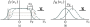
\includegraphics[scale=1]{figures/ch_06/fig_6_1.pdf}
		\caption[]{}
		\label{fig:6_1}
	\end{center}
	\vspace{-0.8cm}
\end{figure}

If the velocity of the charge is much smaller than $c$ ($v\ll c$), then the retardation time $\tau$ will
be negligibly small. In this case, we can consider that the value of $\vec{B}$ at the moment $t$ is determined by the position of the charge at the same moment $t$. If this condition is observed, then
\begin{equation}\label{eq:6_17}
    \vec{B}(P,t) = f\{q, \vec{v}, \vec{r}(t)\}
\end{equation}

\noindent
[we remind our reader that $\vec{v}=\text{constant}$, therefore, $\vec{v}(t-\tau)=\vec{v}(t)$].

The form of function \eqref{eq:6_17} can be established only experimentally. But before giving the results of experiments, let us try to find the logical form of this relation. The simplest assumption is that the magnitude of the vector $\vec{B}$ is proportional to the charge $q$ and the velocity $v$ (when $\vec{v}\to 0$, a magnetic field is absent). We have to ``construct'' the vector $\vec{B}$ we are interested in from the scalar $q$ and the two given vectors $\vec{v}$ and $\vec{r}$. This can be done by vector multiplication of the given vectors and then by multiplying their product by the scalar. The result is the expression
\begin{equation}\label{eq:6_18}
    q (\vecprod{v}{r}).
\end{equation}

\noindent
The magnitude of this expression grows with an increasing distance from the charge (with increasing $r$). It is improbable that the characteristic of a field will behave in this way---for the fields that we know (electrostatic, gravitational), the field does not grow with an increasing distance from the source, but, on the contrary, weakens, varying in proportion to $1/r^2$. Let us assume that the magnetic field of a moving charge behaves in the same way when $r$ changes. We can obtain an inverse proportion to the square of $r$ by dividing \eqn{6_18} by $r^3$. The result is
\begin{equation}\label{eq:6_19}
    \frac{q (\vecprod{v}{r})}{r^3}.
\end{equation}

Experiments show that when $v\ll c$, the magnetic induction of the field of a moving charge is determined by the formula
\begin{equation}\label{eq:6_20}
    \vec{B} = k' \frac{q (\vecprod{v}{r})}{r^3},
\end{equation}

\noindent
where $k'$ is a proportionality constant.

We must stress once more that the reasoning which led us to expression \eqref{eq:6_19} must by no means be considered as the derivation of \eqn{6_20}. This reasoning does not have conclusive force. Its aim is to help us understand and memorize \eqn{6_20}. This equation itself can be obtained only experimentally.

It can be seen from \eqn{6_20} that the vector $\vec{B}$ at every point $P$ is directed at right angles to the plane passing through the direction of the vector $\vec{v}$ and point $P$, so that rotation in the direction of $\vec{B}$ forms a right-handed system with the direction of $\vec{v}$ (see the circle with the dot in \eqn{6_1}). We must note that $\vec{B}$ is a pseudo vector. The value of the proportionality constant $k'$ depends on our choice of the units of the quantities in \eqn{6_20}. This equation is written in the rationalized form as follows:
\begin{equation}\label{eq:6_21}
    \vec{B} = \frac{\mu_0}{4\pi} \frac{q (\vecprod{v}{r})}{r^3}.
\end{equation}

\noindent
This equation can be written in the form
\begin{equation}\label{eq:6_22}
    \vec{B} = \frac{\mu_0}{4\pi} \frac{q (\vec{v}\times\vecuni{r})}{r^3}
\end{equation}

\noindent
[compare with \eqn{1_15}]. It must be noted that in similar equations when $\varepsilon_0$ is in the denominator, $\mu_0$ is in the numerator, and vice versa.

The SI unit of magnetic induction is called the \textbf{tesla} (\si{\tesla}) in honour of the Croatian electrician and inventor Nikola Tesla (1856-1943).

The units of the magnetic induction $B$ are chosen in the cgse and cgsm systems so that the constant $k'$ in \eqn{6_20} equals unity. Hence, the same relation holds between the units of $B$ in these systems as between the units of charge:
\begin{equation}\label{eq:6_23}
    1 \cgs{m}{B} = \num{3e10} \cgs{e}{B}
\end{equation}

\noindent
[see \eqn{6_8}].

The cgsm unit of magnetic induction has a special name---the \textbf{gauss} (\si{\gauss}).

The German mathematician Karl Gauss (1777-1855) proposed a system of units in which all the electrical quantities (charge, current, electric field strength, etc.) are measured in cgse units, and all the magnetic quantities (magnetic induction, magnetic moment, etc.) in cgsm units. This system of units was named the \textbf{Gaussian} one, in honour of its author.

In the Gaussian system, owing to \eqns{6_9}{6_10}, all the equations containing the current or charge in addition to magnetic quantities include one multiplier $1/c$ for each quantity $I$ or $q$ in the relevant equation. This multiplier converts the value of the pertinent quantity ($I$ or $q$) expressed in cgse units to a value expressed in cgsm units (the cgsm system of units is constructed so that the proportionality constants in all the equations equal $1$). For example, in the Gaussian system, \eqn{6_20} has the form
\begin{equation}\label{eq:6_24}
    \vec{B} = \frac{1}{c} \frac{q (\vecprod{v}{r})}{r^3}.
\end{equation}

We must note that the appearance of a preferred direction in space (the direction of the vector $\vec{v}$) when a charge moves leads to the electric field of the moving charge also losing its spherical symmetry and becoming axially symmetrical. The relevant calculations show that the $\vec{E}$ lines of the field of a freely moving charge have the form shown in \fig{6_2}. The vector $\vec{E}$ at point $P$ is directed along the position vector $\vec{r}$ drawn from the point where the charge is at the given moment to point $P$. The magnitude of the field strength is determined by the equation
\begin{equation}\label{eq:6_25}
    E = \frac{1}{4\pi\varepsilon_0} \frac{q}{r^2} \frac{1 - \parenthesis{v^2/c^2}}{\bracket{1 - \parenthesis{v^2/c^2}\sin^2\theta}^{3/2}},
\end{equation}

\noindent
where $\theta$ is the angle between the direction of the velocity $\vec{v}$ and the position vector $\vec{r}$.

\begin{figure}[t]
	\begin{center}
		
\includegraphics[scale=1]{figures/ch_06/fig_6_2.pdf}
		\caption[]{}
		\label{fig:6_2}
	\end{center}
	\vspace{-0.8cm}
\end{figure}

When $v\ll c$, the electric field of a freely moving charge at each moment of time does not virtually differ from the electrostatic field set up by a stationary charge at the point where the moving charge is at the given moment. It must be remembered, however, that this ``electrostatic'' field moves together with the charge. Hence, the field at each point of space changes with time.

At values of $v$ comparable with $c$, the field in directions at right angles to $\vec{v}$ is appreciably stronger than in the direction of motion at the same distance from the charge (see \fig{6_2} drawn for $v/c=0.8$). The field ``flattens out'' in the direction of motion and is concentrated mainly near a plane passing through the charge and perpendicular to the vector $\vec{v}$.

\section{The Biot-Savart Law}\label{sec:6_4}

Let us determine the nature of the magnetic field set up by an arbitrary thin wire through which a current flows. We shall consider a small element of the wire of length $\deriv{l}$. This element contains $nS\, \deriv{l}$ current carriers ($n$ is the number of carriers in a unit volume, and $S$ is the cross-sectional area of the wire where the element $\deriv{l}$ has been taken). At the point whose position relative to the element $\deriv{l}$ is determined by the position vector $\vec{r}$ (\fig{6_3}), a separate carrier of current $e$ sets up a field with the induction
\begin{equation*}
    \vec{B} = \frac{\mu_0}{4\pi} \frac{e [(\vec{v} + \vec{u}) \times \vec{r}]}{r^3}
\end{equation*}

\noindent
[see \eqn{6_21}]. Here, $\vec{v}$ is the velocity of
chaotic motion, and $\vec{u}$ is the velocity of ordered motion of the carrier.

\begin{figure}[t]
	\begin{center}
		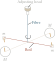
\includegraphics[scale=1]{figures/ch_06/fig_6_3.pdf}
		\caption[]{}
		\label{fig:6_3}
	\end{center}
	\vspace{-0.8cm}
\end{figure}

The value of the magnetic induction averaged over the current carriers in the element $\deriv{l}$ is
\begin{equation*}
    \average{\vec{B}} = \frac{\mu_0}{4\pi} \frac{e [(\average{\vec{v}} + \average{\vec{u}}) \times \vec{r}]}{r^3} = \frac{\mu_0}{4\pi} \frac{e (\average{\vec{u}} \times \vec{r})}{r^3}
\end{equation*}

\noindent
($\average{\vec{v}}=0$). Multiplying this expression by the number of carriers in an element of the wire (equal to $nS\, \deriv{l}$), we get the contribution to the field introduced by the element $\deriv{l}$:
\begin{equation*}
    \deriv{\vec{B}} = \average{\vec{B}} n S\, \deriv{l} = \frac{\mu_0}{4\pi} \frac{S [(ne\average{\vec{u}}) \times \vec{r}]\, \deriv{l}}{r^3}
\end{equation*}

\noindent
(we have put the scalar multipliers $n$ and $e$ inside the sign of the vector product). Taking into account that $ne\average{\vec{u}}=\vec{j}$, we can write
\begin{equation}\label{eq:6_26}
    \deriv{\vec{B}} = \frac{\mu_0}{4\pi} \frac{S (\vecprod{j}{r})\, \deriv{l}}{r^3}.
\end{equation}

Let us introduce the vector $\deriv{\vec{l}}$ directed along the axis of the current element $\deriv{l}$ in the same direction as the current. The magnitude of this vector is $\deriv{l}$. Since the directions of the vectors $\vec{j}$ and $\deriv{\vec{l}}$ coincide, we can write the equation
\begin{equation}\label{eq:6_27}
    \vec{j}\, \deriv{l} = j\, \deriv{\vec{l}}.
\end{equation}

\noindent
Performing such a substitution in \eqn{6_26}, we get
\begin{equation*}
    \deriv{\vec{B}} = \frac{\mu_0}{4\pi} \frac{S j (\deriv{\vec{l}}\times\vec{r})}{r^3}.
\end{equation*}

\noindent
Finally, taking into account that the product $Sj$ gives the current $I$ in the wire, we arrive at the final expression determining the magnetic induction of the field set up by a current element of length $\deriv{l}$:
\begin{equation}\label{eq:6_28}
    \deriv{\vec{B}} = \frac{\mu_0}{4\pi} \frac{I (\deriv{\vec{l}}\times\vec{r})}{r^3}.
\end{equation}

We have derived \eqn{6_28} from \eqn{6_21}. Equation \eqref{eq:6_28} was actually established experimentally before \eqn{6_21} was known. Moreover, the latter equation was derived \eqn{6_28}.

In 1820, the French physicists Jean Biot (1774-1862) and Felix Savart (1791-1841) studied the magnetic fields flowing along thin wires of various shape. The French astronomer and mathematician Pierre Laplace (1749-1827) analysed the experimental data obtained and found that the magnetic field of any current can be calculated as the vector sum (superposition) of the fields set up by the separate elementary sections of the currents. Laplace obtained \eqn{6_28} for the magnetic induction of the field set up by a current element of length $\deriv{l}$. In this connection, \eqn{6_28} is called the \textbf{Biot-Savart-Laplace law}, or more briefly the \textbf{Biot-Savart law}. A glance at \fig{6_3} shows that the vector $\deriv{\vec{B}}$ is directed at right angles to the plane passing through $\deriv{\vec{l}}$ and the point for which the field is being calculated so that rotation about $\deriv{\vec{l}}$ in the direction of $\deriv{\vec{B}}$ is associated with $\deriv{\vec{l}}$ by the right-hand screw rule.
The magnitude of $\deriv{\vec{B}}$ is determined by the expression
\begin{equation}\label{eq:6_29}
    \deriv{B} = \frac{\mu_0}{4\pi} \frac{I\, \deriv{l}\, \sin\theta}{r^3},
\end{equation}

\noindent
where $\alpha$ is the angle between the vectors $\deriv{\vec{l}}$ and $\vec{r}$.

Let us use \eqn{6_28} to calculate the field of a line current, \ie, the field set up by a current flowing through a thin straight wire of infinite length (\fig{6_4}). All the vectors $\deriv{\vec{B}}$ at a given point have the same direction (in our case beyond the drawing). Therefore, addition of the vectors $\deriv{\vec{B}}$ may be replaced with addition of their magnitudes. The point for which we are calculating the magnetic induction is at the distance $b$ from the wire.

\begin{figure}[t]
	\begin{center}
		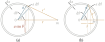
\includegraphics[scale=1]{figures/ch_06/fig_6_4.pdf}
		\caption[]{}
		\label{fig:6_4}
	\end{center}
	\vspace{-0.8cm}
\end{figure}

Inspection of \fig{6_4} shows that
\begin{equation*}
    r = \frac{b}{\sin\alpha},\quad \deriv{l} = \frac{r\, \deriv{\alpha}}{\sin\alpha} = \frac{b\, \deriv{\alpha}}{\sin^2\alpha}.
\end{equation*}

\noindent
Let us introduce these values into \eqn{6_29}:
\begin{equation*}
    \deriv{B} = \frac{\mu_0}{4\pi} \frac{Ib\, \deriv{\alpha} \sin\alpha \sin^2\alpha}{b^2 \sin^2\alpha} = \frac{\mu_0}{4\pi} \frac{I}{b} \sin\alpha\, \deriv{\alpha}.
\end{equation*}

The angle $\alpha$ varies within the limits from $0$ to $\pi$ for all the elements of an infinite line current. Hence,
\begin{equation*}
    B = \int \deriv{B} = \frac{\mu_0}{4\pi} \frac{I}{b} \int_0^{\pi} \sin\alpha\, \deriv{\alpha} = \frac{\mu_0}{4\pi} \frac{2I}{b}.
\end{equation*}

\noindent
Thus, the magnetic induction of the field of a line current is determined by the formula
\begin{equation}\label{eq:6_30}
    B = \frac{\mu_0}{4\pi} \frac{2I}{b}.
\end{equation}

The magnetic induction lines of the field of a line current are a system of concentric circles surrounding the wire (\fig{6_5}).

\begin{figure}[t]
	\begin{center}
		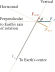
\includegraphics[scale=1]{figures/ch_06/fig_6_5.pdf}
		\caption[]{}
		\label{fig:6_5}
	\end{center}
	\vspace{-0.8cm}
\end{figure}

\section{The Lorentz Force}\label{sec:6_5}

A charge moving in a magnetic field experiences a force which we shall call \textbf{magnetic}. The force is determined by the charge $q$, its velocity $\vec{v}$, and the magnetic induction $\vec{B}$ at the point where the charge is at the moment of time being considered. The simplest assumption is that the magnitude of the force $F$ is proportional to each of the three quantities $q$, $v$, and $B$. In addition, $F$ can be expected to depend on the mutual orientation of the vectors $\vec{v}$ and $\vec{B}$. The direction of the vector $\vec{F}$ should be determined by those of the vectors $\vec{v}$ and $\vec{B}$.

To ``construct'' the vector $\vec{F}$ from the scalar $q$ and the vectors $\vec{v}$ and $\vec{B}$, let us find the vector product of $\vec{v}$ and $\vec{B}$ and then multiply the result obtained by the scalar $q$. The result is the expression
\begin{equation}\label{eq:6_31}
    q (\vecprod{v}{B}).
\end{equation}

It has been established experimentally that the force $\vec{F}$ acting on a charge moving in a magnetic field is determined by the formula
\begin{equation}\label{eq:6_32}
    \vec{F} = k q (\vecprod{v}{B}),
\end{equation}

\noindent
where $k$ is a proportionality constant depending on the choice of the units for the quantities in the formula.

It must be borne in mind that the reasoning which led us to expression \eqref{eq:6_31} must by no means be considered as the derivation of \eqn{6_32}. This reasoning does not have conclusive force. Its aim is to help us memorize \eqn{6_32}. The correctness of this equation can be established only experimentally.

We must note that \eqn{6_32} can be considered as a definition of the magnetic induction $\vec{B}$.

The unit of magnetic induction $\vec{B}$---the tesla----is determined so that the proportionality constant $k$ in \eqn{6_32} equals unity. Hence, in SI units, this equation becomes
\begin{equation}\label{eq:6_33}
    \vec{F} = q (\vecprod{v}{B}).
\end{equation}

The magnitude of the magnetic force is
\begin{equation}\label{eq:6_34}
    F = q v B \sin\alpha,
\end{equation}

\noindent
where $\alpha$ is the angle between the vectors $\vec{v}$ and $\vec{B}$. It can be seen from \eqn{6_34} that a charge moving along the lines of a magnetic field does not experience the action of a magnetic force.

The magnetic force is directed at right angles to the plane containing the vectors $\vec{v}$ and $\vec{B}$. If the charge $q$ is positive, then the direction of the force coincides with that of the vector $\vecprod{v}{B}$. When $q$ is negative, the directions of the vectors $\vec{F}$ and $\vecprod{v}{B}$ are opposite (\fig{6_6}).

Since the magnetic force is always directed at right angles to the velocity of a charged particle, it does no work on the particle. Hence, we cannot change the energy of a charged particle by acting on it with a constant magnetic field.

\begin{figure}[t]
	\begin{center}
		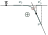
\includegraphics[scale=1]{figures/ch_06/fig_6_6.pdf}
		\caption[]{}
		\label{fig:6_6}
	\end{center}
	\vspace{-0.8cm}
\end{figure}

The force exerted on a charged particle that is simultaneously in an electric and a magnetic field is
\begin{equation}\label{eq:6_35}
    \vec{F} = q \vec{E} + q (\vecprod{v}{B}).
\end{equation}

\noindent
This expression was obtained from the results of experiments by the Dutch physicist Hendrik Lorentz (1853-1928) and is called the \textbf{Lorentz force}.

Assume that the charge $q$ is moving with the velocity $\vec{v}$ parallel to a straight infinite wire along which the current $I$ flows (\fig{6_7}).

According to \eqns{6_30}{6_34}, the charge in this case experiences a magnetic force whose magnitude is
\begin{equation}\label{eq:6_36}
    F = qvB = qv \frac{\mu_0}{4\pi} \frac{2I}{b},
\end{equation}

\noindent
where $b$ is the distance from the charge to the wire. The force is directed toward the wire when the charge is positive if the directions of the current and motion of the charge are the same, and away from the wire if these directions are opposite (see \fig{6_7}). When the charge is negative, the direction of the force is reversed, the other conditions being equal.

Let us consider two like point charges $q_1$ and $q_2$ moving along parallel straight lines with the same velocity $v$ that is much smaller than $c$ (\fig{6_8}). When $v\ll c$, the electric field does not virtually differ from the field of stationary charges (see \sect{6_3}). Therefore, the magnitude of the electric force $\ab{F}{e}$ exerted on the charges can be considered equal to
\begin{equation}\label{eq:6_37}
    \ab{F}{e,$1$} = \ab{F}{e,$2$} = \ab{F}{e} = \frac{1}{4\pi\varepsilon_0} \frac{q_1 q_2}{r^2}.
\end{equation}

\begin{figure}[t]
	\begin{minipage}[t]{0.48\linewidth}
		\begin{center}
			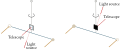
\includegraphics[scale=1]{figures/ch_06/fig_6_7.pdf}
			\caption[]{}
			\label{fig:6_7}
		\end{center}
	\end{minipage}
	\hfill{ }%space{-0.05cm}
	\begin{minipage}[t]{0.48\linewidth}
		\begin{center}
			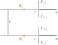
\includegraphics[scale=1]{figures/ch_06/fig_6_8.pdf}
			\caption[]{}
			\label{fig:6_8}
		\end{center}
	\end{minipage}
\vspace{-0.4cm}
\end{figure}

Equations \eqref{eq:6_21} and \eqref{eq:6_3} give us the following expression for the magnetic force $\ab{F}{m}$ exerted on the charges:
\begin{equation}\label{eq:6_38}
    \ab{F}{m,$1$} = \ab{F}{m,$2$} = \ab{F}{m} = \frac{\mu_0}{4\pi} \frac{q_1 q_2 v^2}{r^2}
\end{equation}

\noindent
(the position vector $\vec{r}$ is perpendicular to $\vec{v}$).

Let us find the ratio between the magnetic and electric forces. It follows from \eqns{6_37}{6_38} that
\begin{equation}\label{eq:6_39}
    \frac{\ab{F}{m}}{\ab{F}{e}} = \varepsilon_0 \mu_0 v^2 = \frac{v^2}{c^2}
\end{equation}

[see \eqn{6_15}]. We have obtained \eqn{6_39} on the assumption that $v\ll c$. This ratio holds, however, with any $v$'s.

The forces $\ab{\vec{F}}{e}$ and $\ab{\vec{F}}{m}$ are directed oppositely. Figure \ref{fig:6_8} has been drawn for like and positive charges. For like negative charges, the directions of the forces will remain the same, while the directions of the vectors $\vec{B}_1$ and $\vec{B}_2$ will be reversed. For unlike charges, the directions of the electric and magnetic forces will be the reverse of those shown in the figure.

Inspection of \eqn{6_39} shows that the magnetic force is weaker than the Coulomb one by a factor equal to the square of the ratio of the speed of the charge to that of light. The explanation is that the
magnetic interaction between moving charges is a relativistic effect (see \sect{6_7}). Magnetism would disappear if the speed of light were infinitely great.

\section{Ampere's Law}\label{sec:6_6}

If a wire carrying a current is in a magnetic field, then each of the current carriers experiences the force
\begin{equation}\label{eq:6_40}
    \vec{F} = e [(\vec{v} + \vec{u}) \times \vec{B}]
\end{equation}

\noindent
[see \eqn{6_33}]. Here, $\vec{v}$ is the velocity of chaotic motion of a carrier, and $\vec{u}$ is the velocity of ordered motion. The action of this force is transferred from a current carrier to the conductor along which it is moving. As a result, a force acts on a wire with current in a magnetic field.

Let us find the value of the force $\deriv{\vec{F}}$ exerted on an element of a wire of length $\deriv{l}$. We shall average \eqn{6_40} over the current carriers contained in the element $\deriv{l}$:
\vspace{-12pt}
\begin{equation}\label{eq:6_41}
    \average{\vec{F}} = e [(\average{\vec{v}} + \average{\vec{u}}) \times \vec{B}] = e (\average{\vec{u}} \times \vec{B})
\end{equation}

\noindent
($\vec{B}$ is the magnetic induction at the place where the element $\deriv{l}$ is). The wire element contains $nS\,\deriv{l}$ carriers ($n$ is the number of carriers in unit volume, and $S$ is the cross-sectional area of the wire at the given place). Multiplying \eqn{6_41} by the number of carriers, we find the force we are interested in:
\begin{equation*}
    \deriv{\vec{F}} = \average{\vec{F}} n S\, \deriv{l} = [(ne\average{\vec{u}}) \times \vec{B}] S\, \deriv{l}.
\end{equation*}

\noindent
Taking into account that $ne\average{\vec{u}}$ is the current density $\vec{j}$, and $S\,\deriv{l}$ gives the volume of a wire element $\deriv{V}$, we can write
\begin{equation}\label{eq:6_42}
    \deriv{\vec{F}} = (\vecprod{j}{B})\, \deriv{V}.
\end{equation}

\noindent
Hence, we can obtain an expression for the density of the force, \ie, for the force acting on unit volume of the conductor
\begin{equation}\label{eq:6_43}
    \ab{\vec{F}}{u.v} = \vecprod{j}{B}.
\end{equation}

Let us write \eqn{6_42} in the form
\begin{equation*}
    \deriv{\vec{F}} = (\vecprod{j}{B}) S\, \deriv{l}.
\end{equation*}

\noindent
Replacing in accordance with \eqn{6_27} $\vec{j}S\,\deriv{l}$ with $jS\,\deriv{\vec{l}}= I\,\deriv{\vec{l}}$, we arrive at the equation
\begin{equation}\label{eq:6_44}
    \deriv{\vec{F}} = I (\deriv{\vec{l}} \times \vec{B}).
\end{equation}

\noindent
This equation determines the force exerted on a current element $\deriv{\vec{l}}$ in a magnetic field. Equation \eqref{eq:6_44} was established experimentally by Ampere and is called \textbf{Ampere's law}.

We have obtained Ampere's law on the basis of \eqn{6_33} for the magnetic force. The expression for the magnetic force was actually obtained from the experimentally established equation \eqref{eq:6_44}.

The magnitude of the force \eqref{eq:6_44} is calculated by the equation
\begin{equation}\label{eq:6_45}
    \deriv{F} = I B\, \deriv{l}\, \sin\alpha,
\end{equation}

\noindent
where $\alpha$ is the angle between the vectors $\deriv{\vec{l}}$ and $\vec{B}$ (\fig{6_9}). The force is normal to the plane containing the vectors $\deriv{\vec{l}}$ and $\vec{B}$.

\begin{figure}[t]
	\begin{minipage}[t]{0.35\linewidth}
		\begin{center}
			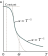
\includegraphics[scale=1]{figures/ch_06/fig_6_9.pdf}
			\caption[]{}
			\label{fig:6_9}
		\end{center}
	\end{minipage}
	\hfill{ }%space{-0.05cm}
	\begin{minipage}[t]{0.59\linewidth}
		\begin{center}
			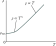
\includegraphics[scale=1]{figures/ch_06/fig_6_10.pdf}
			\caption[]{}
			\label{fig:6_10}
		\end{center}
	\end{minipage}
\vspace{-0.4cm}
\end{figure}

Let us use Ampere's law to calculate the force of interaction between two parallel infinitely long line currents in a vacuum. If the distance between the currents is $b$ (\fig{6_10}), then each element of the current $I_2$ will be in a magnetic field whose induction is $B_1=(\mu_0/4\pi)(2I_1/b)$ [see \eqn{6_30}]. The angle $\alpha$ between the elements of the current $I_2$ and the vector $\vec{B}_1$ is a right one. Hence, according to \eqn{6_45}, the force acting on unit length of the current $I_2$ is
\begin{equation}\label{eq:6_46}
    \ab{F}{21,u} = I_2 B_1 = \frac{\mu_0}{4\pi} \frac{2 I_1 I_2}{b}.
\end{equation}

\noindent
Equation \eqref{eq:6_46} coincides with \eqn{6_2}.

We get a similar equation for the force $\ab{F}{21,u}$ exerted on unit length of the current $I_1$. It is easy to see that when the currents flow in the same direction they attract each other, and in the opposite direction repel each other.

\section{Magnetism as a Relativistic Effect}\label{sec:6_7}

There is a deep relation between electricity and magnetism. On the basis of the postulates of the theory of relativity and of the invariance of an electric charge, we can show that the magnetic interaction of charges and currents is a corollary of Coulomb's law. We shall show this on the example of a charge moving parallel to an infinite line current with the velocity $v_0$\footnote{We have used the symbol $v_0$ for the velocity of a charge to make the notation similar to that in Chap. 8 of Vol. I.} (\fig{6_11}).

According to \eqn{6_36}, the magnetic force acting on a charge in the case being considered is
\begin{equation}\label{eq:6_47}
    F = q v_0 \frac{\mu_0}{4\pi} \frac{2 I}{b}
\end{equation}

\noindent
(the meaning of the symbols is clear from \fig{6_11}). The force is directed toward the conductor carrying the current ($q>0$). Before commencing to derive \eqn{6_47} for the force on the basis of Coulomb's law and relativistic relations, let us consider the following effect. Assume that we have an infinite linear train of point charges of an identical magnitude $e$ spaced a very small distance $l_0$ apart (\fig{6_12}). Owing to the smallness of $l_0$, we can speak of the linear density of the charges $\lambda_0$ which obviously is
\begin{equation}\label{eq:6_48}
    \lambda_0 = \frac{e}{l_0}.
\end{equation}

\begin{figure}[t]
	\begin{minipage}[t]{0.48\linewidth}
		\begin{center}
			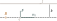
\includegraphics[scale=1]{figures/ch_06/fig_6_11.pdf}
			\caption[]{}
			\label{fig:6_11}
		\end{center}
	\end{minipage}
	\hfill{ }%space{-0.05cm}
	\begin{minipage}[t]{0.48\linewidth}
		\begin{center}
			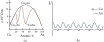
\includegraphics[scale=1]{figures/ch_06/fig_6_12.pdf}
			\caption[]{}
			\label{fig:6_12}
		\end{center}
	\end{minipage}
\vspace{-0.4cm}
\end{figure}

\noindent
Let us bring the charges into motion along the train with the identical velocity $u$. The distance between the charges will therefore diminish and become equal to
\begin{equation*}
    l = l_0 \bracket{1 - \frac{u^2}{c^2}}^{1/2}
\end{equation*}

\noindent
[see Eq. 8.19 of Vol. I]. The magnitude of the charges owing to their invariance, however, remains the same. As a result, the linear density of the charges observed in the reference frame relative to which the charges are moving will change and become equal to
\begin{equation}\label{eq:6_49}
    \lambda = \frac{e}{l} = \frac{\lambda_0}{\sqrt{1 - \parenthesis{u^2/v^2}}}.
\end{equation}

Now let us consider in the reference frame K two infinite trains formed by charges of the same magnitude, but of opposite signs, moving in opposite directions with the same velocity $u$ and virtually coinciding with each other (\fig{6_13}a). The combination of these trains is equivalent to an infinite line current having the value
\begin{equation}\label{eq:6_50}
    I = 2 \lambda u = \frac{2 \lambda_0 u}{\sqrt{1 - \parenthesis{u^2/v^2}}},
\end{equation}

\noindent
where $\lambda$ is the quantity determined by \eqn{6_49}. The total linear density of the charges of a train equals zero, therefore an electric field is absent. The charge $q$ experiences a magnetic force whose magnitude according to \eqns{6_47}{6_50} is
\begin{equation}\label{eq:6_51}
    F = q v_0 \frac{\mu_0}{4\pi} \frac{4 \lambda_0 u}{b \sqrt{1 - \parenthesis{u^2/v^2}}}.
\end{equation}

\begin{figure}[t]
	\begin{center}
		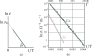
\includegraphics[scale=1]{figures/ch_06/fig_6_13.pdf}
		\caption[]{}
		\label{fig:6_13}
	\end{center}
	\vspace{-0.8cm}
\end{figure}

Let us pass over to the reference frame K$'$ relative to which the charge $q$ is at rest (\fig{6_13}b). In this frame, the charge $q$ also experiences a force (let us denote it by $F'$). This force cannot be of a magnetic origin, however, because the charge $q$ is stationary. The force $F'$ has a purely electrical origin. It appears because the linear densities of the positive and negative charges in the trains are now different (we shall see below that the density of the negative charges is greater). The surplus negative charge distributed over a train sets up an electric field that acts on the positive charge $q$ with the force $F'$ directed toward the train (see \fig{6_13}b).

Let us calculate the force $F'$ and convince ourselves that it ``equals'' the force $F$ determined by \eqn{6_51}. We have taken the word ``equals'' in quotation marks because force is not an invariant quantity. Upon transition from one inertial reference frame to another, the force transforms according to a quite complicated law. In a particular case, when the force $\vec{F}'$ is perpendicular to the relative velocity of the frames K and K' ($\vec{F}' \perp \vec{v}_0$), the transformation has the form
\begin{equation*}
    \vec{F} = \frac{\vec{F}' \sqrt{1 - \parenthesis{v_0^2/c^2}} + \vec{v}_0 (\vec{F}'\ccdot\vec{v}')/c^2}{1 + (\vec{v}_0\ccdot\vec{v}')/c^2}
\end{equation*}

\noindent
($\vec{v}'$ is the velocity of a particle experiencing the force $\vec{F}'$ and measured in the frame K'). If $\vec{v}'=0$ (which occurs in the problem we are considering), the formula for transformation of the force is as follows:
\begin{equation*}
    \vec{F} = \vec{F}' \bracket{1 - \parenthesis{ \frac{v_0^2}{c^2} }}^{1/2}.
\end{equation*}

A glance at this formula shows that the force perpendicular to $\vec{v}_0$ exerted on a particle at rest in the frame K' is also perpendicular to the vector $\vec{v}_0$ in the frame K. The magnitude of the force in this case, however, is transformed by the formula
\begin{equation}\label{eq:6_52}
    F = F' \bracket{1 - \parenthesis{ \frac{v_0^2}{c^2} }}^{1/2}.
\end{equation}

The densities of the charges in the positive and negative trains measured in the frame K' have the values [see \eqn{6_49}]
\begin{equation}\label{eq:6_53}
    \lambda_+' = \frac{\lambda_0}{\sqrt{1 - \parenthesis{u_+'^2/c^2}}},\quad \lambda_-' = - \frac{\lambda_0}{\sqrt{1 - \parenthesis{u_-'^2/c^2}}},
\end{equation}

\noindent
where $u_+'$ and $u_-'$ are the velocities of the charges $+e$ and $-e$ measured in the frame K'. Upon a transition from the frame K to the frame K', the projection of the velocity of a particle onto the direction $x$ coinciding with the direction of $\vec{v}_0$ is transformed by the equation
\begin{equation*}
    u_x' = \frac{u_x - v_0}{1 - \parenthesis{u_xv_0/c^2}}
\end{equation*}

\noindent
[see Eqs. (8.28) of Vol. I; we have substituted $u$ and $u'$ for $v$ and $v'$]. For the charges $+e$, the component $u_x$ equals $u$, for the charges $-e$ it equals $-u$ (see \fig{6_13}a). Hence,
\begin{equation*}
    \parenthesis{u_x'}_+ = \frac{u - v_0}{1 - \parenthesis{uv_0/c^2}},\quad \parenthesis{u_x'}_- = \frac{-u - v_0}{1 + \parenthesis{uv_0/c^2}}.
\end{equation*}

\noindent
Since the remaining projections equal zero, we get
\begin{equation}\label{eq:6_54}
    u_+' = \frac{|u - v_0|}{1 - \parenthesis{uv_0/c^2}},\quad u_-' = \frac{u + v_0}{1 + \parenthesis{uv_0/c^2}}.
\end{equation}

To simplify our calculations, let us pass over to relative velocities:
\begin{equation*}
    \beta_0 = \frac{v_0}{c},\quad \beta = \frac{u}{c},\quad \beta_+' = \frac{u_+'}{c},\quad \beta_- = \frac{u_-'}{c}.
\end{equation*}

\noindent
Equations \eqref{eq:6_53} and \eqref{eq:6_54} therefore acquire the form
\begin{align}
    \lambda_+' &= \frac{\lambda_0}{\sqrt{1 - \beta_+'^2}},\quad \lambda_- = \frac{\lambda_0}{\sqrt{1 - \beta_-'^2}} \label{eq:6_55}\\
    \beta_+' &= \frac{|\beta - \beta_0|}{1 - \beta \beta_0},\quad \beta_-' = \frac{\beta + \beta_0}{1 + \beta \beta_0}.
\end{align}

\noindent
With account taken of these equations, we get the following expression for the total density of the charges:
\begin{align*}
    \lambda' &= \lambda_+' + \lambda_-'\\
    &= \frac{\lambda_0}{\bracket{ 1 - \parenthesis{ \dfrac{\beta-\beta_0}{1-\beta\beta_0} }^2}^{1/2}} - \frac{\lambda_0}{\bracket{ 1 - \parenthesis{ \dfrac{\beta+\beta_0}{1+\beta\beta_0} }^2}^{1/2}}\\
    &= \frac{\lambda_0 \parenthesis{1-\beta\beta_0}}{\sqrt{\parenthesis{1-\beta\beta_0}^2 - \parenthesis{\beta-\beta_0}^2}} - \frac{\lambda_0 \parenthesis{1+\beta\beta_0}}{\sqrt{\parenthesis{1+\beta\beta_0}^2 - \parenthesis{\beta+\beta_0}^2}}.
\end{align*}

\noindent
It is easy to see that
\begin{equation*}
    \parenthesis{1-\beta\beta_0}^2 - \parenthesis{\beta-\beta_0}^2 = \parenthesis{1+\beta\beta_0}^2 - \parenthesis{\beta+\beta_0}^2 = \parenthesis{1-\beta_0^2} \parenthesis{1+\beta^2}.
\end{equation*}

\noindent
Consequently,
\begin{equation}\label{eq:6_57}
    \lambda' = \frac{-2 \lambda_0 \beta \beta_0}{\sqrt{\parenthesis{1-\beta_0^2} \parenthesis{1+\beta^2}}} = \frac{-2 \lambda_0 u v_0}{c^2 \sqrt{1 - \parenthesis{v_0^2/c^2}} \sqrt{1 - \parenthesis{u^2/c^2}}}.
\end{equation}

In accordance with \eqn{1_122}, an infinitely long filament carrying a charge of density $\lambda'$ sets up a field whose strength at the distance $b$ from the filament is
\begin{equation*}
    E' = \frac{1}{2\pi\varepsilon_0} \frac{\lambda'}{b}.
\end{equation*}

\noindent
In this field, the charge $q$ experiences the force
\begin{equation*}
    F' = q E' = \frac{q \lambda'}{2\pi\varepsilon_0 b}.
\end{equation*}

\noindent
Introduction of \eqn{6_57} yields (we have omitted the minus sign)
\begin{align}
    F' &= \frac{q\lambda_0 u v_0}{ \pi\varepsilon_0 vc^2 \sqrt{1 - \parenthesis{v_0^2/c^2}} \sqrt{1 - \parenthesis{u^2/c^2}} } \nonumber\\
    &= qv_0 \frac{\mu_0}{4\pi} \frac{4\lambda_0 u}{\sqrt{1 - \parenthesis{u^2/c^2}}} \frac{1}{\sqrt{1 - \parenthesis{v_0^2/c^2}}} \label{eq:6_58}
\end{align}

\noindent
[we remind our reader that $\mu_0=1/(\varepsilon_0c^2)$; see \eqn{6_15}].

The expression obtained differs from \eqn{6_51} only in the factor $\sqrt{1 - \parenthesis{v_0^2/c^2}}$. We can, therefore, write that
\begin{equation*}
    F = F' \bracket{ 1 - \parenthesis{\frac{v_0^2}{c^2}} }^{1/2},
\end{equation*}

\noindent
where $F$ is the force determined by \eqn{6_51}, and $F'$ is the force determined by \eqn{6_58}. A comparison with \eqn{6_52} shows that $F$ and $F'$ are the values of the same force determined in the frames K and K'.

We must note that in the frame $K'$, which would move relative to the frame K with a velocity differing from that of the charge $v_0$, the force exerted on the charge would consist of both electric and magnetic forces.

The results we have obtained signify that an electric and a magnetic field are inseparably linked with each other and form a single electromagnetic field. Upon a special choice of the reference frame, a field may be either purely electric or purely magnetic. Relative to other reference frames, however, the same field is a combination of an electric and a magnetic field.

In different inertial reference frames, the electric and magnetic fields of the same collection of charges are different. A derivation beyond the scope of a general course in physics leads to the following equations for the transformation of fields when passing over from a reference frame K to a reference frame K' moving relative to it with the velocity $\vec{v}_0$:
\begin{equation}\label{eq:6_59}
    \begin{cases}
        & \!\!\!\!\! E_x' = E_x,\quad E_y = \dfrac{E_y-v_0B_z}{\sqrt{1-\beta^2}},\quad E_z' = \dfrac{E_z+v_0B_y}{\sqrt{1-\beta^2}},\\
        & \!\!\!\!\! B_x' = B_x,\quad B_y = \dfrac{B_y+v_0E_z}{\sqrt{1-\beta^2}},\quad B_z' = \dfrac{B_z-v_0E_y}{\sqrt{1-\beta^2}}.
    \end{cases}
\end{equation}

Here, $E_x$, $E_y$, $E_z$, $B_x$, $B_y$, $B_z$ are the components of the vectors $\vec{E}$ and $\vec{B}$ characterizing an electromagnetic field in the frame K, similar primed symbols are the components of the vectors $\vec{E}'$ and $\vec{B}'$ characterizing the field in the frame K'. The Greek letter $\beta$ stands for the ratio $v_0/c$.

Resolving the vectors $\vec{E}$ and $\vec{B}$, and also $\vec{E}'$ and $\vec{B}'$, into their components
parallel to the vector $\vec{v}_0$ (and, consequently, to the axes $x$ and $x'$) and perpendicular to this vector (\ie, representing, for example, $\vec{E}$ in the form $\vec{E}=\vec{E}_{\parallel}+\vec{E}_{\perp}$, etc.), we can write Eqs. \eqref{eq:6_59} in the vector form:
\begin{equation}\label{eq:6_60}
    \begin{cases}
        & \!\!\!\!\! \vec{E}_{\parallel}' = \vec{E}_{\parallel},\quad \vec{E}_{\perp}' = \dfrac{\vec{E}_{\perp} + (\vec{v}_0 \times \vec{B}_{\perp})}{\sqrt{1-\beta^2}},\\
        & \!\!\!\!\! \vec{B}_{\parallel}' = \vec{B}_{\parallel},\quad \vec{B}_{\perp}' = \dfrac{\vec{B}_{\perp}- \parenthesis{1/c^2} (\vec{v}_0 \times \vec{E}_{\perp})}{\sqrt{1-\beta^2}}.
    \end{cases}
\end{equation}

\noindent
In the Gaussian system of units, Eqs. \eqref{eq:6_60} have the form
\begin{equation}\label{eq:6_61}
    \begin{cases}
        & \!\!\!\!\! \vec{E}_{\parallel}' = \vec{E}_{\parallel},\quad \vec{E}_{\perp}' = \dfrac{\vec{E}_{\perp} + \parenthesis{1/c} (\vec{v}_0 \times \vec{B}_{\perp})}{\sqrt{1-\beta^2}},\\
        & \!\!\!\!\! \vec{B}_{\parallel}' = \vec{B}_{\parallel},\quad \vec{B}_{\perp}' = \dfrac{\vec{B}_{\perp}- \parenthesis{1/c} (\vec{v}_0 \times \vec{E}_{\perp})}{\sqrt{1-\beta^2}}.
    \end{cases}
\end{equation}

\noindent
When $\beta\ll 1$ (\ie, $v_0\ll c$), Eqs. \eqref{eq:6_60} are simplified as follows:
\begin{align*}
    \vec{E}_{\parallel}' &= \vec{E}_{\parallel},\quad \vec{E}_{\perp}' = \vec{E}_{\perp} + \vec{v}_0 \times \vec{B}_{\perp},\\
    \vec{B}_{\parallel}' &= \vec{B}_{\parallel},\quad \vec{B}_{\perp}' = \vec{B}_{\perp}-\parenthesis{1/c^2} (\vec{v}_0 \times \vec{E}_{\perp}).
\end{align*}

\noindent
Adding these equations in pairs, we get
\begin{equation}\label{eq:6_62}
    \begin{cases}
        & \!\!\!\!\! \vec{E}' = \vec{E}_{\parallel}' + \vec{E}_{\perp}' = \vec{E}_{\parallel} + \vec{E}_{\perp} + (\vec{v}_0 \times \vec{B}_{\perp}) = \vec{E} + (\vec{v}_0 \times \vec{B}_{\perp}),\\
        & \!\!\!\!\! \vec{B}' = \vec{B}_{\parallel}' + \vec{B}_{\perp}' = \vec{B}_{\parallel} + \vec{B}_{\perp} - \dfrac{1}{c^2} (\vec{v}_0 \times \vec{E}_{\perp}) = \vec{B} + \dfrac{1}{c^2} (\vec{v}_0 \times \vec{E}_{\perp}).
    \end{cases}
\end{equation}

Since the vectors $\vec{v}_0$ and $\vec{B}_{\parallel}$ are collinear, their vector product equals zero. Hence, $\vec{v}_0 \times \vec{B} = \vec{v}_0 \times \vec{B}_{\parallel} + \vec{v}_0 \times \vec{B}_{\perp} = \vec{v}_0 \times \vec{B}_{\perp}$.
Similarly, $\vec{v}_0 \times \vec{E} = \vec{v}_0 \times \vec{E}_{\perp}$. With this taken into account, Eqs. \eqref{eq:6_62} can be given the form
\begin{equation}\label{eq:6_63}
    \vec{E}' = \vec{E} + \vec{v}_0 \times \vec{B},\quad \vec{B}' = \vec{B} - \dfrac{1}{c^2} (\vec{v}_0 \times \vec{E}).
\end{equation}

\noindent
Fields are transformed by means of these equations if the relative velocity of the reference frames $v_0$ is much smaller than the speed of light in a vacuum $c$ ($v_0\ll c$).

Equations \eqref{eq:6_63} acquire the following form in the Gaussian system of units:
\begin{equation}\label{eq:6_64}
    \vec{E}' = \vec{E} + \dfrac{1}{c} (\vec{v}_0 \times \vec{B}),\quad \vec{B}' = \vec{B} - \dfrac{1}{c} (\vec{v}_0 \times \vec{E}).
\end{equation}

In the example in the frame K considered at the beginning of this section, in which the charge $q$  travelled with the velocity $\vec{v}_0$ parallel to a current-carrying wire, there was only the magnetic field $\vec{B}_{\perp}$ perpendicular to $\vec{v}_0$; the components $\vec{B}_{\parallel}$, $\vec{E}_{\perp}$. and $\vec{E}_{\parallel}$ equalled zero.
According to Eqs. \eqref{eq:6_60} in the frame K', in which the charge $q$ is at rest (this frame travels relative to K with the velocity $\vec{v}_0$), the component $\vec{B}_{\perp}'$ equal to $\vec{B}_{\perp}/\sqrt{1-\beta^2}$ is observed and, in addition, the perpendicular component of the electric field $\vec{E}_{\perp}'=(\vec{v}_0 \times \vec{B}_{\perp})/\sqrt{1-\beta^2}$.

In the frame K, the charge experiences the force
\begin{equation}\label{eq:6_65}
    \vec{F} = q (\vec{v}_0 \times \vec{B}_{\perp}).
\end{equation}

\noindent
Since the charge $q$ is at rest in the frame K', it experiences in this frame only the electric force
\begin{equation}\label{eq:6_66}
    \vec{F}' = q \vec{E}_{\perp}' = \frac{q (\vec{v}_0 \times \vec{B}_{\perp})}{\sqrt{1-\beta^2}}.
\end{equation}

\noindent
A comparison of \eqns{6_65}{6_66} yields $\vec{F} = \vec{F}' \sqrt{1-\beta^2}$, which coincides with \eqn{6_52}.

\section{Current Loop in a Magnetic Field}\label{sec:6_8}

Let us see how a loop carrying a current behaves in a magnetic field. We shall begin with a homogeneous field ($\vec{B}=\text{constant}$). According to \eqn{6_44}, a loop element $\deriv{\vec{l}}$ experiences the force
\begin{equation}\label{eq:6_67}
    \deriv{\vec{F}} = I (\upd\vecprod{l}{B}).
\end{equation}

\noindent
The resultant of such forces is
\begin{equation}\label{eq:6_68}
    \vec{F} = \oint I (\upd\vecprod{l}{B}).
\end{equation}

\noindent
Putting the constant quantities $I$ and $\vec{B}$ outside the integral, we get
\begin{equation*}
    \vec{F} = I \bracket{ \parenthesis{\oint \deriv{\vec{l}} } \times \vec{B} }.
\end{equation*}

\noindent
The integral $\oint\deriv{\vec{l}}$ equals zero, therefore, $\vec{F}=0$. Thus, the resultant force exerted on a current loop in a homogeneous magnetic field equals zero. This holds for loops of any shape (including non-planar ones) with an arbitrary arrangement of the loop relative to the direction of the field. Only homogeneity of the field is essential for the resultant force to equal zero.

In the following, we shall limit ourselves to a consideration of plane loops. Let us calculate the resultant torque set up by the forces \eqref{eq:6_67} applied to a loop. Since the sum of these forces equals zero in a homogeneous field, the resultant torque relative to any point will be the same. Indeed, the resultant torque relative to point $0$ is determined by the expression
\begin{equation*}
    \vec{T} = \int (\vec{r} \times \deriv{\vec{F}}),
\end{equation*}

\noindent
where $\vec{r}$ is the position vector drawn from point $0$ to the point of application of the force $\deriv{\vec{F}}$. Let us take point $0'$ displaced relative to $0$ by the distance $b$. Hence, $\vec{r}=\vec{b}+\vec{r}'$, and accordingly $\vec{r}'=\vec{r}-\vec{b}$. Therefore, the resultant torque relative to point $0'$ is
\begin{align*}
    \vec{T}' &=  \int (\vec{r}' \times \deriv{\vec{F}}) = \int ([\vec{r} - \vec{b}] \times \deriv{\vec{F}}) = \int (\vec{r} \times \deriv{\vec{F}}) - \int (\vec{b} \times \deriv{\vec{F}})\\
    &= \vec{T} - \bracket{ \vec{b} \times \int \deriv{\vec{F}} } = \vec{T},
\end{align*}

\noindent
$\int\deriv{\vec{F}}=0$. The torques calculated relative to two arbitrarily taken points $0$ and $0'$ were found to coincide. We, thus, conclude that the torque does not depend on the selection of the point relative to which it is taken (compare with a couple of forces).

\begin{figure}[t]
	\begin{center}
		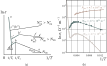
\includegraphics[scale=1]{figures/ch_06/fig_6_14.pdf}
		\caption[]{}
		\label{fig:6_14}
	\end{center}
	\vspace{-0.8cm}
\end{figure}

Let us consider an arbitrary plane current loop in a homogeneous magnetic field $\vec{B}$. Assume that the loop is oriented so that a positive normal to the loop $\hatvec{n}$ is at right angles to the vector $\vec{B}$ (\fig{6_14}). A normal is called positive if its direction is associated with that of the current in the loop by the right-hand screw rule.

Let us divide the area of the loop into narrow strips of width $\deriv{y}$ parallel to the direction of the vector $\vec{B}$ (see \fig{6_14}a; \fig{6_14}b is an enlarged view of one of these strips). The force $\deriv{\vec{F}}_1$ directed beyond the drawing is exerted on the loop element $\deriv{\vec{l}}_1$ enclosing the strip at the left. The magnitude of this force is $\deriv{F}_1 = IB\, \deriv{l}_1\, \sin\alpha_1 = IB\, \deriv{y}$ (see \fig{6_14}b).
The force $\deriv{\vec{F}}_2$ directed toward us is exerted on the loop element $\deriv{\vec{l}}_2$ enclosing the strip at the right. The magnitude of this force is $\deriv{F}_2 = IB\, \deriv{l}_2\, \sin\alpha_2 = IB\, \deriv{y}$.

The result we have obtained signifies that the forces applied to opposite loop elements $\deriv{\vec{l}}_1$ and $\deriv{\vec{l}}_2$ form a
couple whose torque is
\begin{equation*}
    \deriv{T} = I B x\, \deriv{y} = I B\, \deriv{S}
\end{equation*}

\noindent
($\deriv{S}$ is the area of a strip). A glance at \fig{6_14} shows that the vector $\deriv{\vec{T}}$ is perpendicular to the vectors $\hatvec{n}$ and $\vec{B}$ and, consequently, can be written in the form
\begin{equation*}
    \deriv{\vec{T}} = I (\hatvec{n} \times \vec{B})\, \deriv{S}.
\end{equation*}

\noindent
Summation of this equation over all the strips yields the torque acting on the loop:
\begin{equation}\label{eq:6_69}
    \vec{T} = \int I (\hatvec{n} \times \vec{B})\, \deriv{S} = I (\hatvec{n} \times \vec{B}) \int \deriv{S} = I (\hatvec{n} \times \vec{B})\, \deriv{S}
\end{equation}

\noindent
(the field is assumed to be homogeneous, therefore, the product $\hatvec{n}\times\vec{B}$ is the same for all the strips and can be put outside the integral). The quantity $S$ in \eqn{6_69} is the area of the loop.

Equation \eqref{eq:6_69} can be written in the form
\begin{equation}\label{eq:6_70}
    \vec{T} = (I S \hatvec{n}) \times \vec{B}.
\end{equation}

\noindent
This equation is similar to \eqn{1_58} determining the torque exerted on an electric dipole in an electric field. The analogue of $\vec{E}$ in \eqn{6_70} is the vector $\vec{B}$, and that of the electric dipole moment $\vec{p}$ is the expression $IS\hatvec{n}$. This served as the grounds to call the quantity
\begin{equation}\label{eq:6_71}
    \ab{\vec{p}}{m} = I S \hatvec{n}
\end{equation}

\noindent
the \textbf{magnetic dipole moment} of a current loop. The direction of the vector $\ab{\vec{p}}{m}$ coincides with that of a positive normal to the loop.

Using the notation of \eqn{6_71}, we can write \eqn{6_70} as follows:
\begin{equation}\label{eq:6_72}
    \vec{T} = \ab{\vec{p}}{m} \times \vec{B}\quad (\ab{\vec{p}}{m} \perp \vec{B}).
\end{equation}

\begin{figure}[t]
	\begin{center}
		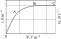
\includegraphics[scale=1]{figures/ch_06/fig_6_15.pdf}
		\caption[]{}
		\label{fig:6_15}
	\end{center}
	\vspace{-0.8cm}
\end{figure}

Now, let us assume that the direction of the vector $\vec{B}$ coincides with that of a positive normal to the loop $\hatvec{n}$ and, therefore, with that of the vector $\ab{\vec{p}}{m}$ too (\fig{6_15}). In this case, the forces exerted on different elements of the loop are in one plane---that of the loop. The force exerted on the loop element $\deriv{\vec{l}}$ is determined by \eqn{6_67}. Let us calculate the resultant torque produced by such forces relative to point $0$ in the plane of the loop:
\begin{equation*}
    \vec{T} = \int \deriv{\vec{T}} = \int (\vec{r} \times \deriv{\vec{F}}) = I \oint [\vec{r} \times (\deriv{\vec{l}} \times \vec{B})]
\end{equation*}

\noindent
($\vec{r}$ is the position vector drawn from point $0$ to the element $\deriv{\vec{l}}$). Let us transform the integrand by means of Eq. (1.35) of Vol. I. The result is
\begin{equation*}
    \vec{T} = I \bracket{ \oint (\vecdot{r}{B})\, \deriv{\vec{l}} - \oint \vec{B} (\vec{r} \ccdot \deriv{\vec{l}}) }.
\end{equation*}

The first integral equals zero because the vectors $\vec{r}$ and $\vec{B}$ are mutually perpendicular. The scalar product inside the second integral is $r\,\deriv{r} = \deriv{\parenthesis{r^2}}/2$. The second integral can, therefore, be written in the form
\begin{equation*}
    \frac{1}{2} \vec{B} \oint \deriv{\parenthesis{r^2}}.
\end{equation*}

\noindent
The total differential of the function $r^2$ is inside the integral. The sum of the increments of a function along a closed path is zero. Hence, the second addend in the expression for $\vec{T}$ is zero too. We have, thus, proved that the resultant torque $\vec{T}$ relative to any point $0$ in the plane of the loop is zero. The resultant torque relative to all other points has the same value (see above).

Thus, when the vectors $\ab{\vec{p}}{m}$ and $\vec{B}$ have the same direction, the magnetic forces exerted on separate portions of a loop do not tend to turn the loop nor shift it from its position. They only tend to stretch the loop in its plane. If the vectors $\ab{\vec{p}}{m}$ and $\vec{B}$ have opposite directions, the magnetic forces tend to compress the loop.

Assume that the directions of the vectors $\ab{\vec{p}}{m}$ and $\vec{B}$ form an arbitrary angle $\alpha$ (\fig{6_16}). Let us resolve the magnetic induction $\vec{B}$ into two components: $\vec{B}_{\parallel}$ parallel to the vector $\ab{\vec{p}}{m}$ and $\vec{B}_{\perp}$ perpendicular
to it, and consider the action of each component separately. The component $\vec{B}_{\parallel}$ will set up forces stretching or compressing the loop. The component $\vec{B}_{\perp}$ whose magnitude is $B\sin\alpha$ will lead to the appearance of a torque that can be calculated by \eqn{6_72}:
\begin{equation*}
    \vec{T} = \ab{\vec{p}}{m} \times \vec{B}_{\perp}.
\end{equation*}

\begin{figure}[t]
	\begin{center}
		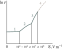
\includegraphics[scale=1]{figures/ch_06/fig_6_16.pdf}
		\caption[]{}
		\label{fig:6_16}
	\end{center}
	\vspace{-0.8cm}
\end{figure}

\noindent
Inspection of \fig{6_16} shows that
\begin{equation*}
    \ab{\vec{p}}{m} \times \vec{B}_{\perp} = \ab{\vec{p}}{m} \times \vec{B}.
\end{equation*}

\noindent
Consequently, in the most general case, the torque exerted on a plane current loop in a homogeneous magnetic field is determined by the equation
\begin{equation}\label{eq:6_73}
    \vec{T} = \ab{\vec{p}}{m} \times \vec{B}.
\end{equation}

\noindent
The magnitude of the vector $\vec{T}$ is
\begin{equation}\label{eq:6_74}
    T = \ab{p}{m} B \sin\alpha.
\end{equation}

To increase the angle a between the vectors $\ab{\vec{p}}{m}$ and $\vec{B}$ by $\deriv{\alpha}$, the following work must be done against the forces exerted on a loop in a magnetic field:
\begin{equation}\label{eq:6_75}
    \deriv{A} = T\, \deriv{\alpha} = \ab{p}{m} B \sin\alpha\, \deriv{\alpha}.
\end{equation}

\noindent
Upon turning to its initial position, a loop can return the work spent for its rotation by doing it on some other body. Hence, the work \eqref{eq:6_75} goes to increase the potential energy $\ab{W}{p,mech}$ which a current loop has in a magnetic field, by the magnitude
\begin{equation*}
    \deriv{\ab{W}{p,mech}} = \ab{p}{m} B \sin\alpha\, \deriv{\alpha}.
\end{equation*}

\noindent
Integration yields
\begin{equation*}
    \ab{W}{p,mech} = - \ab{p}{m} B \cos\alpha + \text{constant}.
\end{equation*}

\noindent
Assuming that $\text{constant}=0$, we get the following expression:
\begin{equation}\label{eq:6_76}
    \ab{W}{p,mech} = - \ab{p}{m} B \cos\alpha = - \ab{\vec{p}}{m} \ccdot \vec{B}
\end{equation}

\noindent
[compare with \eqn{1_61}].

Parallel orientation of the vectors $\ab{\vec{p}}{m}$ and $\vec{B}$ corresponds to the minimum energy \eqref{eq:6_76} and, consequently, to the position of stable equilibrium of a loop.

The quantity expressed by \eqn{6_76} is not the total potential energy of a current loop, but only the part of it that is due to the existence of the torque \eqref{eq:6_73}. To stress this, we have provided the symbol of the potential energy expressed by \eqn{6_76} with the subscript ``mech''. Apart from $\ab{W}{p,mech}$, the total potential energy of a loop includes other addends.

Now let us consider a plane current loop in an inhomogeneous magnetic field. For simplicity, we shall first consider the loop to be circular. Assume that the field changes the fastest in the direction $x$ coinciding with that of $\vec{B}$ where the centre of the loop is, and that the magnetic moment of the loop is oriented along $\vec{B}$ (\fig{6_17}a).

\begin{figure}[t]
	\begin{center}
		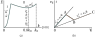
\includegraphics[scale=1]{figures/ch_06/fig_6_17.pdf}
		\caption[]{}
		\label{fig:6_17}
	\end{center}
	\vspace{-0.8cm}
\end{figure}

Here, $\vec{B}\neq\text{constant}$, and \eqn{6_68} does not have to be zero. The force $\deriv{\vec{F}}$ exerted on a loop element is perpendicular to $\vec{B}$, \ie, to the magnetic field line where it intersects $\deriv{\vec{l}}$. Therefore, the forces applied to different loop elements form a symmetrical conical fan (\fig{6_17}b). Their resultant $\vec{F}$ is directed toward a growth in $\vec{B}$ and, therefore, pulls the loop into the region with a stronger field. It is quite obvious that the greater the field changes (the greater is $\diffinpartial{B}{x}$), the smaller is the apex angle of the cone and the greater, other conditions being equal, is the resultant force $\vec{F}$.
If we reverse the direction of the current (now $\ab{\vec{p}}{m}$ is antiparallel to $\vec{B}$), the directions of all the forces $\deriv{\vec{F}}$ and of their resultant $\vec{F}$ will be reversed (\fig{6_17}c). Hence, with such a mutual orientation of the vectors $\ab{\vec{p}}{m}$ and $\vec{B}$, the loop will be pushed out of the field.

It is a simple matter to find a quantitative expression for the force $\vec{F}$ by using \eqn{6_76} for the energy of a loop in a magnetic field. If the orientation of the magnetic moment relative to the field remains constant ($a=\text{constant}$), then $\ab{W}{p,mech}$ will depend only on $x$ (through $B$). Differentiating $\ab{W}{p,mech}$ with respect to $x$ and changing
the sign of the result, we get the projection of the force onto the $x$-axis:
\begin{equation*}
    F_x = - \diffpartial{\ab{W}{p,mech}}{x} = \ab{p}{m} \diffpartial{B}{x} \cos\alpha.
\end{equation*}

\noindent
We assume that the field changes only slightly in the other directions. Hence, we may disregard the projections of the force onto the other axes and assume that $F=F_x$. Thus,
\begin{equation}\label{eq:6_77}
    F = \ab{p}{m} \diffpartial{B}{x} \cos\alpha.
\end{equation}

According to the equation we have obtained, the force exerted on a current loop in an inhomogeneous magnetic field depends on the orientation of the magnetic moment of the loop relative to the direction of the field. If the vectors $\ab{\vec{p}}{m}$ and $\vec{B}$ coincide in direction ($\alpha=0$), then the force is positive, \ie, is directed toward a growth in $vec{B}$ ($\diffinpartial{B}{x}=0$ is assumed to be positive; otherwise, the sign and the direction of the force will be reversed, but the force will pull the loop into the region of a strong field as before). If $\ab{\vec{p}}{m}$ and $\vec{B}$ are antiparallel ($\alpha=\pi$), the force is negative, \ie, directed toward diminishing of $\vec{B}$. We have already obtained this result qualitatively with the aid of \fig{6_17}.

It is quite evident that apart from the force \eqref{eq:6_77}, a current loop in an inhomogeneous magnetic field will also experience the torque \eqref{eq:6_73}.

\section{Magnetic Field of a Current Loop}\label{sec:6_9}

Let us consider the field set up by a current flowing in a thin wire having the shape of a circle of radius $R$ (a ring current). We shall determine the magnetic induction at the centre of the ring current (\fig{6_18}). Every current element produces at the centre an induction directed along a positive normal to the loop. Therefore, vector summation of the $\deriv{\vec{B}}$'s consists in summation of their magnitudes. By \eqn{6_29},
\begin{equation*}
    \deriv{B} = \frac{\mu_0}{4\pi} \frac{I\, \deriv{l}}{R^2}
\end{equation*}

\noindent
($\alpha=\pi/2$). Let us integrate this expression over the entire loop:
\begin{equation*}
    B = \int \deriv{B} = \frac{\mu_0}{4\pi} \frac{I}{R^2} \oint \deriv{l} = \frac{\mu_0}{4\pi} \frac{I}{R^2} 2\pi R = \frac{\mu_0}{4\pi} \frac{2I \parenthesis{\pi R^2}}{R^3}.
\end{equation*}

The expression in parentheses is the magnitude of the magnetic dipole moment $\ab{p}{m}$ [see \eqn{6_71}]. Hence, the magnetic induction at the centre of a ring current has the value
\begin{equation}\label{eq:6_78}
    B = \frac{\mu_0}{4\pi} \frac{2\ab{p}{m}}{R^3}.
\end{equation}

Inspection of \fig{6_18} shows that the direction of the vector $\vec{B}$ coincides with that of a positive normal to the loop, \ie, with that of the vector $\ab{\vec{p}}{m}$. Therefore, \eqn{6_78} can be written in the vector form:
\begin{equation}\label{eq:6_79}
    \vec{B} = \frac{\mu_0}{4\pi} \frac{2\ab{\vec{p}}{m}}{R^3}.
\end{equation}

\begin{figure}[t]
	\begin{minipage}[t]{0.35\linewidth}
		\begin{center}
			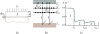
\includegraphics[scale=0.98]{figures/ch_06/fig_6_18.pdf}
			\caption[]{}
			\label{fig:6_18}
		\end{center}
	\end{minipage}
	\hfill{ }%space{-0.05cm}
	\begin{minipage}[t]{0.61\linewidth}
		\begin{center}
			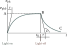
\includegraphics[scale=0.98]{figures/ch_06/fig_6_19.pdf}
			\caption[]{}
			\label{fig:6_19}
		\end{center}
	\end{minipage}
\vspace{-0.4cm}
\end{figure}

Now let us find $\vec{B}$ on the axis of the ring current at the distance of $r$ from the centre of the loop (\fig{6_19}). The vectors $\deriv{\vec{B}}$ are perpendicular to the planes passing through the relevant element $\deriv{\vec{l}}$ and the point where we are seeking the field. Hence, they form a symmetrical conical fan (\fig{6_19}b). We can conclude from considerations of symmetry that the resultant vector $\vec{B}$ is directed along the axis of the loop.
Each of the component vectors $\deriv{\vec{B}}$ contributes $\deriv{\vec{B}_{parallel}}$ equal in magnitude to $\deriv{B}\sin\beta=\deriv{B}(R/b)$ to the resultant vector. The angle $\alpha$ between $\deriv{\vec{l}}$ and $\vec{b}$ is a right one, hence,
\begin{equation*}
    \deriv{B_{\parallel}} = \deriv{B} \frac{R}{b} = \frac{\mu_0}{4\pi} \frac{I\, \deriv{l}}{b^2} \frac{R}{b} = \frac{\mu_0}{4\pi} \frac{I R\, \deriv{l}}{b^3}.
\end{equation*}

\noindent
Integrating over the entire loop and substituting $\sqrt{R^2+r^2}$ for $b$, we obtain
\begin{align}
    B &= \int \deriv{B_{\parallel}} = \frac{\mu_0}{4\pi} \frac{I R}{b^3} \oint \deriv{l} = \frac{\mu_0}{4\pi} \frac{I R}{b^3} 2\pi R = \frac{\mu_0}{4\pi} \frac{2\parenthesis{I \pi R^2}}{\parenthesis{R^2+r^2}^{3/2}} \nonumber\\
    &= \frac{\mu_0}{4\pi} \frac{2 \ab{p}{m}}{\parenthesis{R^2+r^2}^{3/2}}. \label{eq:6_80}
\end{align}

\noindent
This equation determines the magnitude of the magnetic induction on the axis of a ring current. With a view to the vectors $\vec{B}$ and $\ab{\vec{p}}{m}$ having the same direction, we can write \eqn{6_80} in the vector form:
\begin{equation}\label{eq:6_81}
    \vec{B} = \frac{\mu_0}{4\pi} \frac{2 \ab{\vec{p}}{m}}{\parenthesis{R^2+r^2}^{3/2}}.
\end{equation}

\noindent
This expression does not depend on the sign of $r$. Hence, at points on the axis symmetrical relative to the centre of the current, $\vec{B}$ has the same magnitude and direction.

When $r=0$, \eqn{6_81} transforms, as should be expected, into \eqn{6_79} for the magnetic induction at the centre of a ring current.

For great distances from a loop, we may disregard $R^2$ in the denominator in comparison with $r^2$. Equation \eqref{eq:6_81} now becomes
\begin{equation}\label{eq:6_82}
    \vec{B} = \frac{\mu_0}{4\pi} \frac{2 \ab{\vec{p}}{m}}{r^3}\quad (\text{along the current axis}),
\end{equation}

\noindent
which is similar to \eqn{1_55} for the electric field strength along the axis of a dipole.

Calculations beyond the scope of the present book show that a magnetic dipole moment $\ab{\vec{p}}{m}$ can be ascribed to any system of currents or moving charges localized in a restricted portion of space (compare with the electric dipole moment of a system of charges). The magnetic field of such a system at distances that are great in comparison with its dimensions is determined through $\ab{\vec{p}}{m}$ using the same equations as those used to determine the field of a system of charges at great distances through the electric dipole moment (see \sect{1_10}). In particular, the field of a plane loop of any shape at great distances from it is
\begin{equation}\label{eq:6_83}
    B = \frac{\mu_0}{4\pi} \frac{2 \ab{p}{m}}{r^3} \sqrt{1 + 3 \cos^2\theta},
\end{equation}

\noindent
where $r$ is the distance from the loop to the given point, and $\theta$ is the angle between the direction of the vector $\ab{\vec{p}}{m}$ and the direction from the loop to the given point of the field [compare with \eqn{1_53}]. When $\theta=0$, \eqn{6_83} gives the same value as \eqn{6_82} for the magnitude of the vector $\vec{B}$.

\begin{figure}[t]
	\begin{center}
		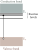
\includegraphics[scale=1]{figures/ch_06/fig_6_20.pdf}
		\caption[]{}
		\label{fig:6_20}
	\end{center}
	\vspace{-0.8cm}
\end{figure}

Figure \ref{fig:6_20} shows the magnetic field lines of a ring current. It shows only the lines in one of the planes passing through the current axis. A similar picture will be observed in any of these planes.

It follows from everything said in the preceding and this sections that the magnetic dipole moment is a very important characteristic of a current loop. It determines both the field set up by a loop and the behaviour of the loop in an external magnetic field.

\section{Work Done When a Current Moves in a Magnetic Field}\label{6_10}

Let us consider a current loop formed by stationary wires and a movable rod of length $l$ sliding along them (\fig{6_21}). Let the loop be in an external magnetic field which we shall assume to be homogeneous and at right angles to the plane of the loop. With the directions of the current and field shown in the figure, the force $\vec{F}$ exerted on the rod will be directed to the right and will equal
\begin{equation*}
    F = I B l.
\end{equation*}

\noindent
When the rod moves to the right by $\deriv{h}$, this force does the positive work
\begin{equation}\label{eq:6_84}
    \deriv{A} = F\, \deriv{h} = I B l\, \deriv{h} = I B\, \deriv{S},
\end{equation}

\noindent
where $\deriv{S}$ is the shaded area (see \fig{6_21}a).

Let us see how the magnetic induction flux $\Phi$ through the area of the loop will change when the rod moves. We shall agree, when calculating the flux through the area of a current loop, that the quantity $\hatvec{n}$ in the equation
\begin{equation*}
    \Phi = \int \vec{B} \ccdot \hatvec{n}\, \deriv{S},
\end{equation*}

\noindent
is a positive normal, \ie, one that forms a right-handed system with the direction of the current in the loop (see \sect{6_8}). Hence, in the case shown in \fig{6_21}a, the flux will be positive and equal to $BS$ ($S$ is the area of the loop). When the rod moves to the right, the area of the loop receives the positive increment $\deriv{S}$. As a result, the flux also receives the positive increment $\deriv{\Phi}=B\,\deriv{S}$. Equation \eqref{eq:6_84} can, therefore, be written in the form
\begin{equation}\label{eq:6_85}
    \deriv{A} = I\, \deriv{\Phi}.
\end{equation}

\begin{figure}[t]
	\begin{center}
		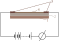
\includegraphics[scale=1.1]{figures/ch_06/fig_6_21.pdf}
		\caption[]{}
		\label{fig:6_21}
	\end{center}
	\vspace{-0.8cm}
\end{figure}

\noindent
When the field is directed toward us (\fig{6_21}b), the force exerted on the rod is directed to the left. Therefore when the rod moves to the right through the distance $\deriv{h}$, the magnetic force does the negative work
\begin{equation}\label{eq:6_86}
    \deriv{A} = - I B l\, \deriv{h} = - I B\, \deriv{S}.
\end{equation}

\noindent
In this case, the flux through the loop is $-BS$. When the area of the loop grows by $\deriv{S}$, the flux receives the increment $\deriv{\Phi}=-B\,\deriv{S}$. Hence, \eqn{6_86} can also be written in the form of \eqn{6_85}.

The quantity $\deriv{\Phi}$ in \eqn{6_85} can be interpreted as the flux through the area covered by the rod when it moves. We can say accordingly that the work done by the magnetic force on a portion of a current loop equals the product of the current and the magnitude of the magnetic flux through the surface covered by this portion during its motion.

Equations \eqref{eq:6_84} and \eqref{eq:6_85} can be combined into a single vector expression. For this purpose, we shall compare the vector $\vec{l}$ having the direction of the current with the rod (\fig{6_22}). Regardless of the direction of the vector $\vec{B}$ (toward us or away from us), the force exerted on the rod can be represented in the form
\begin{equation*}
    \vec{F} = I \vecprod{l}{B}.
\end{equation*}

\noindent
When the rod moves through the distance $\derivec{h}$, the force does the work
\begin{equation*}
    \deriv{A} = \vec{F}\, \derivec{h} = I \vecprod{l}{B}\, \derivec{h}.
\end{equation*}

\noindent
Let us perform a cyclic transposition of the multipliers in this triple scalar product [see Eq. (1.34) of Vol. I]. The result is
\begin{equation}\label{eq:6_87}
    \deriv{A} = I \vec{B} (\derivec{h} \times \vec{l}).
\end{equation}

\begin{figure}[t]
	\begin{center}
		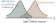
\includegraphics[scale=1.1]{figures/ch_06/fig_6_22.pdf}
		\caption[]{}
		\label{fig:6_22}
	\end{center}
	\vspace{-0.8cm}
\end{figure}

A glance at \fig{6_22} shows that the vector product $(\derivec{h}\times\vec{l})$ equals in magnitude the area $\deriv{S}$ described by the rod during its motion and has the direction of a positive normal $\hatvec{n}$. Hence,
\begin{equation}\label{eq:6_88}
    \deriv{A} = I (\vec{B} \ccdot \hatvec{n})\, \deriv{S}.
\end{equation}

\noindent
In the case shown in \fig{6_22}a, we have $\vec{B}\ccdot\hatvec{n}=B$, and we arrive at \eqn{6_84}. In the case shown in \fig{6_22}b, we have $\vec{B}\ccdot\hatvec{n}=-B$. and we arrive at \eqn{6_86}.

The expression $\vec{B}\ccdot\hatvec{n}\,\deriv{S}$ determines the increment of the magnetic flux through the loop due to motion of the rod. Thus, \eqn{6_88} can be written in the form of \eqref{eq:6_85}. But \eqn{6_88} has an advantage over \eqref{eq:6_85} because we ``automatically'' get the sign of $\deriv{\Phi}$ from it and, consequently, the sign of $\deriv{A}$ too.

Let us consider a rigid current loop of any shape in an arbitrary magnetic field. We shall find the work done upon an arbitrary infinitely small displacement of the loop. Assume that the loop element $\derivec{l}$ was displaced by $\derivec{h}$ (\fig{6_23}). The magnetic force does the following work on it:
\begin{equation}\label{eq:6_89}
    \deriv{\ab{A}{el}} = I (\derivec{l} \times \vec{B}) \ccdot \derivec{h}.
\end{equation}

\noindent
Here, $\vec{B}$ is the magnetic induction at the place where the loop element $\derivec{l}$ is.

Performing a cyclic transposition of the multipliers in \eqn{6_89}, we get
\begin{equation}\label{eq:6_90}
    \deriv{\ab{A}{el}} = I \vec{B} \ccdot (\derivec{h} \times \derivec{l}).
\end{equation}

\noindent
The magnitude of the vector product $\derivec{h} \times\derivec{l}$ equals the area of a parallelogram constructed on the vectors $\derivec{h}$ and $\derivec{l}$, \ie, the area $\deriv{S}$ described by the element $\derivec{l}$ during its motion. The direction of the vector product coincides with that of a positive normal to the area $\deriv{S}$. Consequently,
\begin{equation}\label{eq:6_91}
    \vec{B} \ccdot (\derivec{h} \times \derivec{l}) = (\vec{B} \ccdot \hatvec{n})\, \deriv{S} = \deriv{\ab{\Phi}{el}},
\end{equation}

\noindent
where $\deriv{\ab{\Phi}{el}}$ is the increment of the magnetic flux through the loop due to the displacement of the loop element $\derivec{l}$.

\begin{figure}[t]
	\begin{center}
		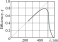
\includegraphics[scale=0.98]{figures/ch_06/fig_6_23.pdf}
		\caption[]{}
		\label{fig:6_23}
	\end{center}
	\vspace{-0.9cm}
\end{figure}

With a view to \eqn{6_91}, we can write \eqn{6_90} in the form
\begin{equation}\label{eq:6_92}
    \deriv{\ab{A}{el}} = I\, \deriv{\ab{\Phi}{el}}.
\end{equation}

\noindent
Summation of \eqn{6_92} over all the loop elements yields an expression for the work of the magnetic forces upon an arbitrary infinitely small displacement of the loop:
\begin{equation}\label{eq:6_93}
    \deriv{A} = \int \deriv{\ab{A}{el}} = \int I \, \deriv{\ab{\Phi}{el}} = I \int \deriv{\ab{\Phi}{el}} = I\, \deriv{\Phi}
\end{equation}

\noindent
($\deriv{\Phi}$ is the total increment of the flux through the loop).

To find the work done upon a finite arbitrary displacement of a loop, let us integrate \eqn{6_93} over the entire loop:
\begin{equation}\label{eq:6_94}
    A_{12} = \int \deriv{A} = I \int \deriv{\ab{\Phi}{el}} = I \parenthesis{\Phi_2 - \Phi_1}.
\end{equation}

\noindent
Here, $\Phi_1$ and $\Phi_2$ are the values of the magnetic flux through the loop in its initial and final positions. The work done by the magnetic forces on the loop thus equals the product of the current and the increment of the magnetic flux through the loop.

In particular, when a plane loop rotates in a homogeneous field from a position in which the vectors $\ab{\vec{P}}{m}$ and $\vec{B}$ are directed oppositely (in this position $\Phi=-BS$) to a position in which these vectors have the same direction (in this position $\Phi=BS$, the magnetic
forces do the following work on the loop:
\begin{equation*}
    A = I [BS - (BS)] = 2 I B S.
\end{equation*}

\noindent
The same result is obtained with the aid of \eqn{6_91} for the potential energy of a loop in a magnetic field:
\begin{equation*}
    A = \ab{W}{init} - \ab{W}{fin} = \ab{p}{m} B - (- \ab{p}{m} B) = 2 \ab{p}{m} B = 2 I S B
\end{equation*}

\noindent
($\ab{p}{m}=IS$).

We must note that the work expressed by \eqn{6_94} is done not at the expense of the energy of the external magnetic field, but at the expense of the source maintaining a constant current in the loop. We shall show in \sect{8_2} that when the magnetic flux through a loop changes, an induced e.m.f. $\ab{\mathcal{E}}{i}=-(\diffin{\Phi}{t})$ is set up in the loop. Hence, the source in addition to the work done to liberate the Joule heat must also do work against the induced e.m.f. determined by the expression
\begin{equation*}
    A = \int \deriv{A} = -\int \ab{\mathcal{E}}{i} l\, \deriv{t} = \int \diffin{\Phi}{t} I\, \deriv{t} = \int I\, \deriv{\Phi} = I (\Phi_2 - \Phi_1),
\end{equation*}

\noindent
that coincides with \eqn{6_94}.

\section{Divergence and Curl of a Magnetic Field}\label{sec:6_11}

The absence of magnetic charges in nature\footnote{The British physicist Paul Dirac made the assumption that magnetic charges (called Dirac's monopoles) should exist in nature. Searches for these charges have meanwhile given no results and the question of the existence of Dirac's...} results in the fact that the lines of the vector $\vec{B}$ have neither a beginning nor an end. Therefore, in accordance with \eqn{1_77}, the flux of the vector $\vec{B}$ through a closed surface must equal zero. Thus, for any magnetic field and an arbitrary closed surface, the condition
\begin{equation}\label{eq:6_95}
    \Phi_B = \oint_S \vec{B}\, \derivec{S} = 0,
\end{equation}

\noindent
is observed. This equation expresses Gauss's theorem for the vector $\vec{B}$: the flux of the magnetic induction vector through any closed surface equals zero.

Substituting a volume integral for the surface one in \eqn{6_95} in accordance with \eqn{1_108}, we find that
\begin{equation*}
    \int_V \divop{\vec{B}}\, \deriv{V} = 0.
\end{equation*}

\noindent
The condition which we have arrived at must be observed for any arbitrarily chosen volume $V$. This is possible only if the integrand at each point of the field is zero. Thus, a magnetic field has the property that its divergence is zero everywhere:
\begin{equation}\label{eq:6_96}
    \divop{\vec{B}} = 0.
\end{equation}

Let us now turn to the circulation of the vector $\vec{B}$. By definition, the circulation equals the integral
\begin{equation}\label{eq:6_97}
    \oint \vec{B} \ccdot \derivec{l}.
\end{equation}

\noindent
It is the simplest to calculate this integral for the field of a line current. Assume that a closed loop is in a plane perpendicular to the current (\fig{6_24}; the current is perpendicular to the plane of the drawing and is directed beyond the drawing). At each point of the loop, the vector $\vec{B}$ is directed along a tangent to the circumference passing through this point. Let us substitute $B\,\deriv{l_B}$ for $\vec{B}\ccdot \derivec{l}$ in the expression for the circulation ($\deriv{l_B}$ is the projection of a loop element onto the direction of the vector $\vec{B}$). Inspection of the figure shows that $\deriv{l_B}$ equals $b\,\deriv{\alpha}$, where $b$ is the distance from the wire carrying the current to $\derivec{l}$, and $\deriv{\alpha}$ is the angle through which a radial straight line turns when it moves along the loop over the element $\derivec{l}$.
Thus, introducing \eqn{6_30} for $B$, we get
\begin{equation}\label{eq:6_98}
    \vec{B} \ccdot \derivec{l} = B\,\deriv{l_B} = \frac{\mu_0}{4\pi} \frac{2I}{b} b\, \deriv{\alpha} = \frac{\mu_0 I}{2\pi}\, \deriv{\alpha}.
\end{equation}

\begin{figure}[t]
	\begin{center}
		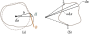
\includegraphics[scale=1.0]{figures/ch_06/fig_6_24.pdf}
		\caption[]{}
		\label{fig:6_24}
	\end{center}
	\vspace{-0.8cm}
\end{figure}

With a view to \eqn{6_98}, we have
\begin{equation}\label{eq:6_99}
    \oint \vec{B} \ccdot \derivec{l} = \frac{\mu_0 I}{2\pi} \oint \deriv{\alpha}.
\end{equation}

\noindent
Upon circumvention of the loop enclosing the current, the radial straight line constantly turns in one direction, therefore, $\oint\deriv{\alpha}= 2\pi$. Matters are different if the current is not enclosed by the loop (\fig{6_24}b). Here, upon circumvention of the loop, the radial straight line first turns in one direction (segment $1$-$2$), and then in the opposite one ($2$-$1$), owing to which $\oint\deriv{\alpha}$ equals zero. With a view to this result. we can write that
\begin{equation}\label{eq:6_100}
    \oint \vec{B} \ccdot \derivec{l} = \mu_0 I,
\end{equation}

\noindent
where $I$ must be understood as the current enclosed by the loop. If the loop does not enclose the current, the circulation of the vector $\vec{B}$ is zero.

The sign of expression \eqref{eq:6_100} depends on the direction of circumvention of the loop (the angle $\alpha$ is measured in the same direction). If the direction of circumvention forms a right-handed system with the direction of the current, quantity \eqref{eq:6_100} is positive, in the opposite case it is negative. The sign can be taken into consideration by assuming $I$ to be an algebraic quantity. A current whose direction is associated with that of circumvention of a loop by the right-hand screw rule must be considered positive; a current of the opposite direction will be negative.

Equation \eqref{eq:6_100} will allow us to easily recall \eqn{6_30} for $B$ of the field of a line current. Imagine a plane loop in the form of a circle of radius $b$ (\fig{6_25}). At each point of this loop, the vector $\vec{B}$ has the same magnitude and is directed along a tangent to the circle. Hence, the circulation equals the product of $B$ and the length of the circumference $2\pi b$, and \eqn{6_100} has the form
\begin{equation*}
    B \times 2\pi b = \mu_0 I.
\end{equation*}

\noindent
Thus, $B=\mu_0 I/(2\pi b)$ [compare with \eqn{6_30}].

\begin{figure}[t]
	\begin{minipage}[t]{0.41\linewidth}
		\begin{center}
			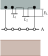
\includegraphics[scale=1]{figures/ch_06/fig_6_25.pdf}
			\caption[]{}
			\label{fig:6_25}
		\end{center}
	\end{minipage}
	\hfill{ }%space{-0.05cm}
	\begin{minipage}[t]{0.55\linewidth}
		\begin{center}
			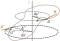
\includegraphics[scale=1]{figures/ch_06/fig_6_26.pdf}
			\caption[]{}
			\label{fig:6_26}
		\end{center}
	\end{minipage}
\vspace{-0.4cm}
\end{figure}

The case of a non-planar loop (\fig{6_26}) differs from that of a plane one considered above, only in that upon motion along the loop the radial straight line not only turns about the wire, but also moves along it. All our reasoning which led us to \eqn{6_100} remains true if we understand $\deriv{\alpha}$ to be the angle through which the projection of the radial straight line onto a plane perpendicular to the current turns. The total angle of rotation of this projection is $2\pi$ if the loop encloses the current, and zero otherwise. We thus again arrive at \eqn{6_100}.

We have obtained \eqn{6_100} for a line current. We can show that it also holds for a current flowing in a wire of an arbitrary shape, for example, for a ring current.

Assume that a loop encloses several wires carrying currents. Owing to the superposition principle [see \eqn{6_16}]:
\begin{equation*}
    \oint \vec{B}\ccdot \derivec{l} = \oint \parenthesis{ \sum_k \vec{B}_k }\, \derivec{l} = \sum_k \oint \vec{B}_k\, \derivec{l}.
\end{equation*}

\noindent
Each of the integrals in this sum equals $\mu_0I_k$. Hence,
\begin{equation}\label{eq:6_101}
    \oint \vec{B}\ccdot \derivec{l} = \mu_0 \sum_k I_k
\end{equation}

\noindent
(remember that $I_k$ is an algebraic quantity).

If currents flow in the entire space where a loop is, the algebraic sum of the currents enclosed by the loop can be represented in the form
\begin{equation}\label{eq:6_102}
    \sum_k I_k = \int_S \vec{j}\ccdot \derivec{S} = \int_S \vec{j}\ccdot \hatvec{n}\, \deriv{S}.
\end{equation}

\noindent
The integral is taken over the arbitrary surface $S$ enclosing the loop. The vector $\vec{j}$ is the current density at the point where area element $\deriv{S}$ is; $\hatvec{n}$ is a positive normal to this element (\ie, a normal forming a right-handed system with the direction of circumvention
of the loop in calculating the circulation).

Substituting \eqn{6_102} for the sum of the currents in \eqn{6_101}, we obtain
\begin{equation*}
    \oint \vec{B}\ccdot \derivec{l} = \mu_0 \int_S \vec{j}\ccdot \derivec{S}.
\end{equation*}

Transforming the left-band side according to Stokes's theorem, we arrive at the equation
\begin{equation*}
    \int_S (\curlop{\vec{B}}) \ccdot \derivec{S} = \mu_0 \int_S \vec{j}\ccdot \derivec{S}.
\end{equation*}

\noindent
This equation must be obeyed with an arbitrary choice of the surface $S$ over which the integrals are taken. This is possible only if the integrands have identical values at every point. We, thus, arrive at the conclusion that the curl of the magnetic induction vector is proportional to the current density vector at the given point:
\begin{equation}\label{eq:6_103}
    \curlop{\vec{B}} = \mu_0 \vec{j}.
\end{equation}

\noindent
The proportionality constant in the SI system is $\mu_0$.

We must note that \eqns{6_101}{6_103} hold only for the field in a vacuum in the absence of time-varying electric fields.

Thus, we have found the divergence and curl of a magnetic field in a vacuum. Let us compare the equations obtained with the similar equations for an electrostatic field in a vacuum. According to Eqs. \eqref{eq:1_112}, \eqref{eq:1_117}, \eqref{eq:6_96} and \eqref{eq:6_103}:
\begin{align*}
    \divop{\vec{E}} = \frac{1}{\varepsilon_0}\rho &\quad \text{(the divergence of $\vec{E}$ equals $\rho$ divided by $\varepsilon_0$)}\\
    \curlop{\vec{E}} = 0 &\quad \text{(the curl of $\vec{E}$ equals zero)}\\
    \divop{\vec{B}} = 0 &\quad \text{(the divergence of $\vec{B}$ equals zero)}\\
    \curlop{\vec{B}} = \mu_0 \vec{j} &\quad \text{(the curl of $\vec{B}$ equals $\mu_0$ multiplied by $\vec{j}$)}.
\end{align*}

A comparison of these equations shows that an electrostatic and a magnetic field are of an appreciably different nature. The curl of an electrostatic field equals zero; consequently, an electrostatic field is potential and can be characterized by the scalar potential $\varphi$. The curl of a magnetic field at points where there is a current differs from zero. Accordingly, the circulation of the vector $\vec{B}$ is proportional to the current enclosed by a loop. This is why we cannot ascribe to a magnetic field a scalar potential that would be related to $\vec{B}$ by an equation similar to \eqn{1_41}. This potential would not be unique---upon each circumvention of the loop and return to the initial point it would receive an increment equal to $\mu_0 I$. A field
whose curl differs from zero is called a \textbf{vortex} or a \textbf{solenoidal} one.

Since the divergence of the vector $\vec{B}$ is zero everywhere, this vector can be represented as the curl of a function $\vec{A}$:
\begin{equation}\label{eq:6_104}
    \vec{B} = \curlop{\vec{A}},
\end{equation}

\noindent
the divergence of a curl always equals zero [see \eqn{1_106}]. The function $\vec{A}$ is called the \textbf{vector potential}. A treatment of the vector potential is beyond the scope of the present book.

\section{Field of a Solenoid and Toroid}\label{sec:6_12}

A solenoid is a wire wound in the form of a spiral onto a round cylindrical body. The magnetic field lines of a solenoid are arranged approximately as shown in \fig{6_27}. The direction of these lines inside the solenoid forms a right-handed system with the direction of the current in the turns.

A real solenoid has a current component along its axis. In addition, the linear density of the current $\ab{j}{lin}$ (equal to the ratio of the current $\deriv{I}$ to an element of solenoid length $\deriv{l}$) changes periodically along the solenoid. The average value of this density is
\begin{equation}\label{eq:6_105}
    \average{\ab{j}{lin}} = \average{\diff{I}{l}} = nI,
\end{equation}

\noindent
where $n$ is the number of solenoid turns per unit length and $I$ the current in the solenoid.

In the science of electromagnetism, a great part is played by an imaginary infinitely long solenoid having no axial current component and, in addition, having a constant linear current density $\ab{j}{lin}$ along its entire length. The reason for this is that the field of such a solenoid is homogeneous and is bounded by the volume of the solenoid (similarly, the electric field of an infinite parallel-plate capacitor is homogeneous and is bounded by the volume of the capacitor).

In accordance with what has been said above, let us imagine a solenoid in the form of an infinite thin-walled cylinder around which flows a current of constant linear density
\begin{equation}\label{eq:6_106}
    \ab{j}{lin} = nI.
\end{equation}

\noindent
Let us divide the cylinder into identical ring currents---``turns''. Examination of \fig{6_28} shows that each pair of turns arranged symmetrically relative to a plane perpendicular to the solenoid axis sets up a magnetic induction parallel to the axis at any point of this plane. Hence, the resultant of the field at any point inside and outside an infinite solenoid can only have a direction parallel to the axis.

It can be seen from \fig{6_27} that the directions of the field inside and outside a finite solenoid are opposite. The directions of the fields do not change when the length of a solenoid is increased, and in the limit, when $l\to\infty$, they remain opposite. In an infinite solenoid, as in a finite one, the direction of the field inside the solenoid forms a right-handed system with the direction in which the current flows around the cylinder.

\begin{figure}[t]
	\begin{minipage}[t]{0.48\linewidth}
		\begin{center}
			\includegraphics[scale=1]{figures/ch_06/fig_6_27b.pdf}
			\caption[]{}
			\label{fig:6_27}
		\end{center}
	\end{minipage}
	\hfill{ }%space{-0.05cm}
	\begin{minipage}[t]{0.48\linewidth}
		\begin{center}
			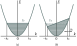
\includegraphics[scale=1]{figures/ch_06/fig_6_28.pdf}
			\caption[]{}
			\label{fig:6_28}
		\end{center}
	\end{minipage}
\vspace{-0.4cm}
\end{figure}

It follows from the vector $\vec{B}$ and the axis being parallel that the field both inside and outside an infinite solenoid must be homogeneous. To prove this, let us take an imaginary rectangular loop $1$-$2$-$3$-$4$ inside a solenoid (\fig{6_29}; $4$-$1$ is along the axis of the solenoid).

Passing clockwise around the loop, we get the value $(B_2 - B_1)a$ for the circulation of the vector $\vec{B}$. The loop does not enclose the currents, therefore the circulation must be zero [see \eqn{6_101}]. Hence, it follows that $\vec{B}_1 = \vec{B}_2$. Arranging section $2$-$3$ of the loop at
any distance from the axis, we shall always find that the magnetic induction $\vec{B}_2$ at this distance equals the induction $\vec{B}_1$ on the solenoid axis. Thus, the homogeneity of the field inside the solenoid has been proved.

Now let us turn to loop $1'$-$2'$-$3'$-$4'$. We have depicted the vectors $\vec{B}_1'$ and $\vec{B}_2'$ by a dash line since, as we shall find out in the following, the field outside an infinite solenoid is zero. Meanwhile, all that we know is that the possible direction of the field outside the solenoid is opposite to that of the field inside it. Loop $1'$-$2'$-$3'$-$4'$ does not enclose the currents; therefore, the circulation of the vector $\vec{B}'$ around this loop, equal to $(B_1' - B_2')a$, must be zero. It thus follows that $\vec{B}_1'=\vec{B}_2'$.
The distances from the solenoid axis to sections $1'$-$4'$ and $2'$-$3'$ were taken arbitrarily. Consequently, the value of $\vec{B}'$ at any distance from the axis will be the same outside the solenoid. Thus, the homogeneity of the field outside the solenoid has been proved too.

The circulation around the loop shown in \fig{6_30} is $a(B+B')$ (for clockwise circumvention). This loop encloses a positive current of magnitude $\ab{j}{lin}a$. In accordance with \eqn{6_101}, the following equation must be observed:
\begin{equation*}
    a(B+B') = \mu_0 \ab{j}{lin} a,
\end{equation*}

\noindent
or after cancelling $a$ and replacing $\ab{j}{lin}$ with $nI$ [see \eqn{6_106}]
\begin{equation}\label{eq:6_107}
    (B+B') = \mu_0 n I.
\end{equation}

\noindent
This equation shows that the field both inside and outside an infinite solenoid is finite.

\begin{figure}[t]
	\begin{minipage}[t]{0.48\linewidth}
		\begin{center}
			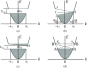
\includegraphics[scale=1]{figures/ch_06/fig_6_29.pdf}
			\caption[]{}
			\label{fig:6_29}
		\end{center}
	\end{minipage}
	\hfill{ }%space{-0.05cm}
	\begin{minipage}[t]{0.48\linewidth}
		\begin{center}
			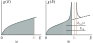
\includegraphics[scale=1]{figures/ch_06/fig_6_30.pdf}
			\caption[]{}
			\label{fig:6_30}
		\end{center}
	\end{minipage}
\vspace{-0.4cm}
\end{figure}

Let us take a plane at right angles to the solenoid axis (\fig{6_31}). Since the field lines $\vec{B}$ are closed, the magnetic fluxes through the inner part $S$ of this plane and through its outer part $S'$ must be the same. Since the fields are homogeneous and normal to the plane, each of the fluxes equals the product of the relevant value of the magnetic induction and the area penetrated by the flux. We, thus, get the expression
\begin{equation*}
    BS = B'S'.
\end{equation*}

The left-hand side of this equation is finite, the factor $S'$ in the right-hand side is infinitely great. Hence, it follows that $B'=0$.

Thus, we have proved that the magnetic induction outside an infinitely long solenoid is zero. The field inside the solenoid is homogeneous. Assuming in \eqn{6_107} that $B' = 0$, we arrive at an equation for the magnetic induction inside a solenoid:
\begin{equation}\label{eq:6_108}
    B = \mu_0 n I.
\end{equation}

The product $nI$ is called the number of ampere-turns per metre. At $n = 1000$ turns per metre and a current of \SI{1}{\ampere}, the magnetic induction inside a solenoid is $4\pi\times\SI{e-4}{\tesla}=4\pi \si{\gauss}$.

The symmetrically arranged turns make an identical contribution to the magnetic induction on the axis of a solenoid [see \eqn{6_81}]. Therefore, at the end of a semi-infinite solenoid, the magnetic induction on its axis equals half the value given by \eqn{6_108}:
\begin{equation}\label{eq:6_109}
    B = \frac{1}{2} \mu_0 n I.
\end{equation}

Practically, if the length of a solenoid is considerably greater than its diameter, \eqn{6_108} will hold for points in the central part of the solenoid, and \eqn{6_109} for points on its axis near its ends.

A toroid is a wire wound onto a body having the shape of a torus (\fig{6_32}). Let us take a loop in the form of a circle of radius $r$ whose centre coincides with that of a toroid. Owing to symmetry,
the vector $\vec{B}$ at every point must be directed along a tangent to the loop. Hence, the circulation of $\vec{B}$ is
\begin{equation*}
    \oint \vec{B} \ccdot \derivec{l} = B \times 2\pi r
\end{equation*}

\noindent
($\vec{B}$ is the magnetic induction at the points through which the loop passes).

\begin{figure}[t]
	\begin{minipage}[t]{0.48\linewidth}
		\begin{center}
			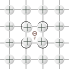
\includegraphics[scale=1]{figures/ch_06/fig_6_31.pdf}
			\caption[]{}
			\label{fig:6_31}
		\end{center}
	\end{minipage}
	\hfill{ }%space{-0.05cm}
	\begin{minipage}[t]{0.48\linewidth}
		\begin{center}
			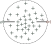
\includegraphics[scale=1]{figures/ch_06/fig_6_32.pdf}
			\caption[]{}
			\label{fig:6_32}
		\end{center}
	\end{minipage}
\vspace{-0.4cm}
\end{figure}

If a loop passes inside a toroid, it encloses the current $2\pi RnI$ ($R$ is the radius of the toroid, and $n$ is the number of turns per unit of its length). In this case,
\begin{equation*}
    B \times 2\pi r = \mu_0 2\pi R n I,
\end{equation*}

\noindent
whence
\begin{equation}\label{eq:6_110}
    B = \mu_0 n I \frac{R}{r}.
\end{equation}

A loop passing outside a toroid encloses no currents, hence, we have $B\times 2\pi r = 0$ for it. Thus, the magnetic induction outside a toroid is zero.

For a toroid whose radius $R$ considerably exceeds the radius of a turn, the ratio $R/r$ for all the points inside the toroid differs only slightly from unity, and instead of \eqn{6_110} we get an equation
coinciding with \eqn{6_108} for an infinitely long solenoid. In this case, the field may be considered homogeneous in each of the toroid sections. The field is directed differently in different sections. We can, therefore, speak of the homogeneity of the field within the entire toroid only conditionally, bearing in mind the identical magnitude of $\vec{B}$.

A real toroid has a current component along its axis. This component sets up a field similar to that of a ring current in addition to the field given by \eqn{6_110}.
